\RequirePackage{ifpdf}
\documentclass[master,tocprelim]{cornell}
%
% tocprelim option must be included to put the roman numeral pages in the
% table of contents
%
% The cornellheadings option will make headings completely consistent with
% guidelines.
%
% This sample document was originally provided by Blake Jacquot, and
% fixed up by Andrew Myers.
%
%Some possible packages to include
\usepackage{graphicx,pstricks}
\usepackage{graphics}
\usepackage{moreverb}
\usepackage{subfigure}
\usepackage{epsfig}
\usepackage{subfigure}
\usepackage{hangcaption}
%\usepackage{txfonts}
\usepackage{palatino}

%new packages added by Yinglei Wang
\usepackage[cmex10]{amsmath}
\usepackage{url}

\def\mywidth{5in}


%if you're having problems with overfull boxes, you may need to increase
%the tolerance to 9999
\tolerance=9999

\bibliographystyle{unsrt}
%\bibliographystyle{IEEEbib}

\renewcommand{\caption}[1]{\singlespacing\hangcaption{#1}\normalspacing}
\renewcommand{\topfraction}{0.85}
\renewcommand{\textfraction}{0.1}
\renewcommand{\floatpagefraction}{0.75}

\title {Flash Memory for Ubiquitous Hardware Security Functions}
\author {Yinglei Wang}
\conferraldate {December}{2013}
\degreefield {M.S.}
\copyrightholder{Yinglei Wang}
\copyrightyear{2013}

\begin{document}

\maketitle
\makecopyright

\begin{abstract}
We demonstrate that unmodified commercial Flash memory can 
provide three important security functions: true random number 
generation, digital fingerprinting and information hiding. Taking advantage of random telegraph 
noise (a type of quantum noise source in highly scaled Flash memory cells) 
enables high quality true random number generation at a rate up to  
10Kbits / second. A scheme based on partial programming exploits process 
variation in threshold voltages to allow quick generation of many unique 
fingerprints that can be used for identification and authentication. 
Information hiding hides 
data within an analog characteristic of Flash, the program time of individual bits. 
Because the technique uses analog behaviors, normal Flash memory operations are
not affected and hidden information is invisible in the data stored in the memory.
Even if an attacker checks a Flash chip's analog characteristics,
experimental results indicate that the hidden information is difficult to distinguish 
from inherent manufacturing variation or normal wear on the device.
Moreover, the hidden data can survive erasure of the Flash memory data.
All
schemes require no change to Flash chips or interfaces, and do not require additional hardware. 
\end{abstract}

\begin{biosketch}
Yinglei Wang attended Peking(Beijing) University in China as an EECS undergraduate student from year 2006 to 2010. 
She entered the MS/PHD program in ECE, Cornell University in Fall, 2010. She worked with Prof. Edwin C. Kan, 
Prof. G. Edward Suh and Prof. Christopher Batten on flash memory security and on-chip network. She will work as
a software engineer at Oracle from January, 2014.
\end{biosketch}

\begin{dedication}
This document is dedicated to my parents and my husband Xuetian Weng, who is now a PHD student in Computer Science.
\end{dedication}

\begin{acknowledgements}
Upon leaving Cornell and Ithaca after spending three years and a half here, I have to admit it is an unexpected ending.
Nevertheless, it is invaluable experience which taught me a lot of things: knowledge, research, relationships and life. 

First, I would like 
to express the deepest appreciation and gratitude to my advisor, Prof. Edwin C. Kan.  He has supported me throughout 
graduate school, and provided the vision and advise necessary to finish my dissertation. More importantly, he gives me the 
freedom to explore new things and tries his best to support me. I would also like to express sincere thanks to my committee member, 
Prof. G. Edward Suh. He has given me so much guidance and help on my research. What's more, he tried to help me in my most 
difficult days, and I really appreciate it. Special thanks to my committee member, Prof. Christopher Batten. 
His computer architecture course is the first computer architecture/organaization course I took and I was deeply attracted to it.
I also learned 
a lot, both technical skills and the methodology of engineering, when working with him. I would also like
to take this opporutnity to express my sincere thanks to one of my course instructors, 
Prof. Jose F. Martinez. In addition to his interesting lectures, He is concerned with my situation and I could feel free to tell him my efforts, worries, concerns and feelings. I really 
appreciate his advice and his attitude towards work and life.

Throughout the years, I have the honor to work with several brilliant graduate and undergradute students. I would like to thank KK Yu, 
Greg Malysa and Shuo Wu for their help and contribution to this topic. I would also like to thank the group memebers, especially 
Kshitij Auluck and Yunfei Ma for their 
inspiring discussions and friendship.

I wish to thank my parents, Deming Wang and Chunhua Wang. Their unconditional love always gives me the warmth and courage to 
carry on. I love them forever. I also hope to thank my husband, Xuetian Weng, who is now a PHD student in Computer Science, Stony Brook 
Unviersity. He can always tolerate my bad temper and complaints. He also encourages me to think about the good things about life 
and be a happy person. I'm so lucky to have his love in my life and I love him. Best wishes to his PHD career.

Sincere thanks and best wishes to all my friends at Cornell.

\end{acknowledgements}

\contentspage
\tablelistpage
\figurelistpage

\normalspacing \setcounter{page}{1} \pagenumbering{arabic}
\pagestyle{cornell} \addtolength{\parskip}{0.5\baselineskip}

\chapter{Introduction}

\section{Overview}
Flash memory has gained a ubiquitous place in the computing landscape today. 
Virtually all mobile devices such as smartphones and tablets rely on Flash 
memory as their non-volatile storage. Flash memory is also moving into laptop 
and desktop computers, intending to replace the mechanical hard drive. 
Floating-gate non-volatile memory is even more broadly used in electronic 
applications with a small amount of non-volatile memory. For example, even 
8-bit or 16-bit microcontrollers for embedded systems commonly have on-chip 
EEPROMs to store instructions and data. Many people also carry Flash memory 
as standalone storage medium as in USB memory sticks and SD cards.

In this paper, we propose to utilize analog behaviors of off-the-shelf Flash 
memory to enable hardware-based security functions in a wide range of electronic 
devices without requiring custom hardware. More specifically, we show that a 
standard Flash memory interface can be used to generate true random numbers 
from quantum and thermal noises and to produce device fingerprints based on 
manufacturing variations.
This paper also introduces a technique to hide information in analog characteristics 
of Flash memory in a way that the hidden bits are not visible at all from the viewpoint of normal 
Flash memory content. Our technique encodes a hidden bit in the program
time of a group of Flash cells; a fast program time encodes bit '1' and a slow program time 
encodes bit '0'. We found that writing 0 into a Flash cell incurs more 
stress on the cell than writing 1, which in turn results in a larger decrease in
the program time of the corresponding cell. While the program time of individual cells cannot
be accurately controlled, our experiments demonstrate that bits can be reliably encoded
in the program time using many cells collectively.
The techniques can be applied to any floating-gate 
non-volatile memory in general, and does not require any hardware modifications 
to today’s Flash memory chips, allowing them to be widely deployed.

\section{Quantum Random Number Generation}
Hardware random number generators (RNGs) provides important foundations 
in building secure systems. For example, true randomness is a critical 
ingredient in many cryptographic primitives and security protocols; random 
numbers are often required to generate secret keys or prevent replays in 
communications. While pseudo-random number generators are often used in today’s 
systems, they cannot provide true randomness if a seed is reused or predictable. 
As an example, a recent study showed that reuse of virtual machine (VM) snapshots 
can break the Transport Level Security (TLS) protocol due to predictable random 
numbers \cite{ristenpart2010good}. Given the importance of a good source of randomness, high security 
systems typically rely on hardware RNGs.
Instead of requiring custom hardware modules for RNGs, we found that analog 
noise in Flash memory bits can be used to reliably generate true random numbers. 
An interesting finding is that the standard Flash chip interface can be used to 
put a memory bit in partially programmed state so that the internal noise can be 
observed through the digital interface. There exist two sources of true randomness 
in Flash bits, Random Telegraph Noise (RTN) and thermal noise. While both sources 
can be leveraged for RNGs, our scheme focuses on RTN, which is quantum noise. Unlike 
thermal noise, which can be reduced significantly at extremely low temperatures, 
RTN behavior continues at all temperature ranges. Moreover, the quantum uncertainty 
nature of RTN provides a better entropy source than system level noises which rely 
on the difficulty of modeling complex yet deterministic systems. Our algorithm 
automatically selects bits with RTN behavior and converts RTN into random binary bits.
Experimental results demonstrate that the RTN behavior exists in Flash memory and 
can be converted into random numbers through the standard Flash interface. The 
Flash-based RNG is tested using the NIST test suite \cite{rukhin2001statistical} and is shown to 
pass all tests successfully. Moreover, we found that the RNG works even 
at a very low temperature (-80 °C). In fact, the RTN behavior is more visible at 
low temperatures.  On our test platform, the Flash RNG generates about 1K 
to 10K bits per second. Overall, the experiments show that true random 
numbers can be generated reliably from off-the-shelf Flash memory chips 
without requiring custom circuits.

\section{Device Fingerprint}

In addition to generating true random numbers, we also found that the standard Flash interface can be used to extract fingerprints (or signatures) that are unique for each Flash chip. For this purpose, our technique exploits inherent random variations during Flash manufacturing processes. More specifically, we show that the distributions of transistor threshold voltages can be measured through the standard Flash interface using incremental partial programming. Experimental results show that these threshold voltage distributions can be used as fingerprints, as they are significantly different from chip to chip, or even from location to location within a chip. The distributions also stay relatively stable across temperature ranges and over time. Thanks to the large number of bits (often several gigabits) in modern Flash chips, this technique can generate a large number of independent fingerprints from each chip. 

The Flash fingerprints provide an attractive way to identify and/or authenticate hardware devices and generate device-specific keys, especially when no cryptographic module is available or a large number of independent keys are desired. For example, at a hardware component level, the fingerprints can be used to distinguish genuine parts from counterfeit components without requiring cryptography to be added to each component. The fingerprinting technique can also be used for other authentication applications such as turning a Flash device into a two-factor authentication token, or identifying individual nodes in sensor networks. 

While the notion of exploiting manufacturing process variations to generate silicon device fingerprints and secret keys is not new and has been extensively studied under the name of Physical Unclonable Functions (PUFs) \cite{suhpuf2007}, the Flash-based technique in this paper represents a unique contribution in terms of its practical applicability. Similar to true RNGs, most PUF designs require custom circuits to convert unique analog characteristics into digital bits. On the other hand, our technique can be applied to off-the-shelf Flash without hardware changes. Researchers have recently proposed techniques to exploit existing bi-stable storage elements such as SRAMs \cite{koeberl2011practical} or Flash cells \cite{trust2011} to generate device fingerprints. Unfortunately, obtaining fingerprints from bi-stable elements requires a power cycle (power off and power on) of a device for every fingerprint generation. The previous approach to fingerprinting Flash only works for a certain types of Flash chips and takes long time (100 seconds for one fingerprint) because it relies on rare errors called program disturbs. As an example, we did not see any program disturbs in SLC Flash chips that we used in experiments. To the best of our knowledge, the proposed device fingerprinting techniques is the first that is fast (less than 1 second for a 1024-bit fingerprint) and widely applicable without interfering with normal operation or requiring custom hardware.

\section{Information Hiding}

This part introduces a technique to hide information in analog characteristics 
of Flash memory in a way that the hidden bits are not visible at all from the viewpoint of normal 
Flash memory content. More specifically, our technique encodes a hidden bit in the program
time of a group of Flash cells; a fast program time encodes bit '1' and a slow program time 
encodes bit '0'. We found that writing 0 into a Flash cell incurs more 
stress on the cell than writing 1, which in turn results in a larger decrease in
the program time of the corresponding cell. While the program time of individual cells cannot
be accurately controlled, our experiments demonstrate that bits can be reliably encoded
in the program time using many cells collectively.

%Technical challenge - partial programming. 

%Main Advantages / Characteristics
While a number of steganography techniques have been developed previously, our
Flash-based technique provides unique benefits compared to typical digital
steganography schemes where information is hidden in another form of digital content such 
as images and documents. In particular, the hidden information in Flash memory is
decoupled from the Flash memory content and instead tied to the physical object.
The following summarizes the main benefits of our scheme compared to
digital steganography.

\begin{itemize}

\item {\bf Covert}: The proposed technique does not change normal Flash operations
or content at all. As a result, inspecting the Flash memory content does not reveal
any hidden information. All Flash memory operations can still be performed without
any change, even with hidden information. In fact, our experimental results suggest 
that even analog characteristics of Flash memory such as page program/erase time do not
change noticeably. 

\item {\bf Erase tolerant}: The hidden information in Flash memory remains intact
even if the entire Flash memory is erased and programmed with new content. In
fact, our experiments show that the hidden information can survive even hundreds
of program/erase operations. 

\item {\bf Copy tolerant}: In typical digital steganography, the cover text with
hidden information can be easily copied and stored so that it can be analyzed 
over time. The hidden information in our technique, however, is tied to physical
Flash memory and can only be accessed by measuring the program time of individual memory 
cells while the Flash memory is in one's possession. Because modern Flash memory chips 
often contain tens or hundreds of billions of memory cells, fully characterizing
a Flash chip without knowing the location of hidden bits is quite time consuming.
%Our experiments estimate that such an attack will take multiple weeks.

\end{itemize}

In a sense, the proposed information hiding technique is similar to physical
steganography methods where information is hidden in physical objects.
% should we cite wikipedia? I included a survey paper instead below. \cite{wikipedia-steg}.
For example, people have used secret inks to write messages on blank parts
of other messages \cite{exploringsteganography}. However, 
the proposed technique provides a couple of key
benefits over traditional physical steganography methods thanks to being
electrical.

\begin{itemize}

\item {\bf No hardware modification}:
The proposed technique works on unmodified Flash chips using the standard
interface. In fact, the technique can be implemented as a software program
as long as a low-level Flash interface is exposed.

\item {\bf High capacity}:
Thanks to the high capacity of Flash memory, our technique provides a fairly
high capacity compared to traditional physical steganography techniques. 
For example, even if we hide one bit for every 512 Flash cells, a 8GB Flash
chip can contain 16MB of hidden information. 

\end{itemize}

%Application?

Given the ubiquity of Flash memory and the easy applicability of the proposed
scheme on commercial Flash chips, we believe that the technique can enable a
number of interesting applications. An obvious application of the information
hiding in Flash is a secure and covert storage of data.
For example, a user can hide sensitive information in the Flash memory of
a smartphone with confidence that others cannot retrieve the information
even when the phone is lost or stolen. Information hiding provides an
additional layer of protection on top of typical encryption by preventing an 
adversary from reading or even copying the ciphertext.

On the other hand, the capability to covertly communicate may be misused to
bypass legitimate access control policies. For example, in the business world,
the hidden information in Flash may be misused to export trade secrets.
In this sense, this study points out the potential danger.

Another traditional application of information hiding is watermarking. 
In particular, given that the hidden information is tied to a physical Flash
memory chip, the proposed technique can be used to embed watermarking
in devices with Flash memory. For example, mobile or embedded devices
may be watermarked to help retrieve them when lost or stolen. Similarly,
the watermarks can be used to distinguish genuine devices from low-quality
counterfeits. 


\chapter{Flash Memory Background} \label{sec:flashbackground}

This section provides background material on Flash memory and
its operating principles to aid understanding of our Flash-based
information hiding scheme.

\section{Floating Gate Transistors}

Flash memory is composed of arrays of floating-gate transistors.
A floating-gate transistor is a transistor with two gates,
stacked on top of each other. One gate is electrically insulated
(floating). Figure~\ref{fig:fgtrans} shows an example of a floating-gate device.
The control gate is on top. An insulated conductor, surrounded
by oxide, is between the control gate and the channel. This
conductor is the floating gate. Information is stored as the
presence or absence of trapped charge on the floating gate. The
trapped negative charge reduces the current flowing through the
channel when the N-type MOS transistor is on. This current
difference is sensed and translated into the appropriate binary
value.


\begin{figure} 
\begin{center} 
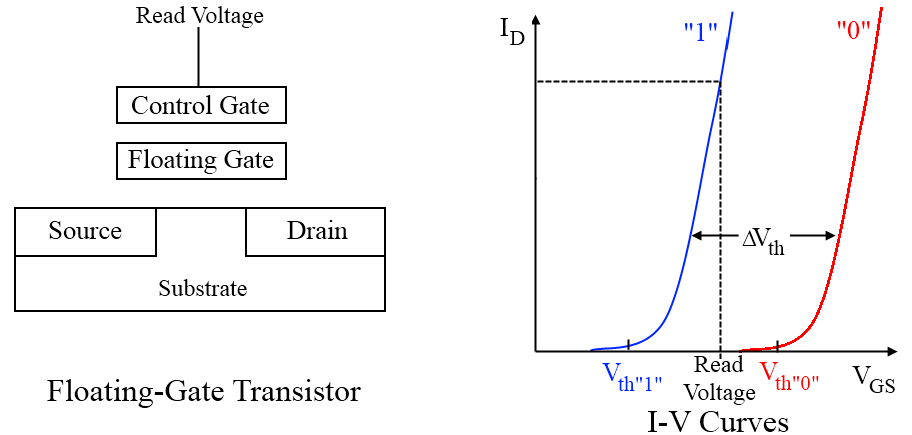
\includegraphics[width=\mywidth]{figs/fgtrans-cleanaxis.png} 
%\includegraphics[width=3.0in]{figs/eval_performance_diff_context.pdf} 
\caption{Flash memory cell based on a floating gate transistor.}
\label{fig:fgtrans} 
%\vspace{-0.25in}
\end{center} 
\end{figure} 

Flash cells without charge on their floating-gate allow full
current flow in the channel and hence are read as a binary ``1''.
The presence of charge on the floating-gate will discourage the
presence of current in the channel, making the cell store a ``0''.
Effectively, the charge on the floating-gate increases the
threshold voltage (Vth) of a transistor. Single-level cells (SLC)
store one bit of information per cell by using two threshold
voltage levels.
Multi-level cells (MLC) store more than one bit by more finely
dividing the threshold voltage levels: for example, four levels 
can be used to store two bits per cell.

%Note that the threshold voltage without any charge on the
%floating-gate is different for each transistor due to variations
%in %manufacturing processes. As a result, the amount of charge
%that needs to be stored to the floating-gate for a cell to
%reliably represent a %''0'' state varies from cell to cell. If
%the threshold voltage is not shifted sufficiently, a cell can be
%in an unreliable (partially %programmed) state that can be
%interpreted as either 1 or 0. In this paper, we exploit the
%threshold voltage variations and the partially %programmed state
%to hide and later to read hidden information.

\section{Flash Organization and Operation}

At a high-level, Flash memory provides three major operations:
read, erase, and program (write). In order to read a bit in a
Flash cell, the corresponding transistor is turned on and the
amount of current is detected. A write to a Flash cell involves
two steps. First, an erase operation pushes charge off the
floating-gate by applying a large negative voltage on the
control gate. Then, a program (write) operation stores charge on
the floating-gate by selectively applying a large positive
voltage if the bit needs to be zero.

An important concept in Flash memory operation is that of pages
and blocks. Pages are the smallest unit in which data is read or
written, and are usually 2KB to 8KB. Blocks are the smallest
unit for an erase operation and made up of several pages,
usually 32 - 128 pages. Note that Flash does not provide
bit-level program or erase. To read an address from a Flash
chip, the page containing the address is read. To update a
value, the block that includes the address must be first erased.
Then, the corresponding page is written with an update and other
pages in the block are restored.

\section{Aging} 

Flash requires high voltages to store and erase information.
The voltages involved place great stress on the device oxide;
each program operation and each erase operation slightly damages the oxide,
wearing out the device.
After thousands of program and erase cycles, the oxide could
have sustained enough damage to render the bit non-operational, leaving
it in a stuck-at state or in a leaky state that cannot reliably 
hold information over a period of time. Flash is usually
guaranteed by the manufacturer up to a certain number of program
and erase cycles. 

Even before failures, the stress causes
the cell's analog characteristics to change. In particular, the
program time that is required to flip a state from '1' to '0' for
a cell tends to reduce as the number of program/erase (PE) cycles increases
for that cell. We exploit this program time shift in order to
hide information.



\section{Partial Programming}

Our information hiding scheme relies on the measurement of program
time, the time it takes to program a Flash cell, at individual cell
granularity. However, the standard Flash memory interface
requires all bits in a page to be programmed together. 
Normally, a program operation on a page is held for a long enough time 
that any cell level variation within a page is overcome. 
Therefore, the normal program time only reveals how long programming
the entire page takes, not how long it takes to program individual bits.

To find the program time on a per-cell basis, we use
a technique called ``partial programming'' \cite{flash-ieeesp2012}.
The standard Flash memory interfaces allow the ``partial program'' 
of a cell by aborting a program operation before completion. 
If the program
operation is interrupted, the Flash cell may be in an unreliable
state that could be interpreted as 1 or 0. Further ``partial
programs'' will accumulate charge on the floating gate and
eventually result in the cell entering a stable programmed
state, as if a full program was applied. Effectively, the number of
partial program operations to flip a bit from 1 to 0 represents
the program time for the bit.
In this sense, we use the ``partial programming'' technique to 
to find program time for individual cells. After a partial program to a
page, we read the page and record the state of each bit. When a
bit changes to the programmed state (from 1 to 0), we
note the number of partial programs required to flip the bit as 
the bit's program time.



\chapter{Random Number Generation} \label{sec:rng}

\section{Theory and Implementation}

\subsection{Random Telegraph Noise (RTN)}

The proposed RNG uses a device effect called Random Telegraph Noise (RTN) as the source of randomness. In general, RTN refers to the alternating capture and emission of carriers at a defect site (trap) of a very small electronic device, which generates discrete variation in the channel current \cite{kirton1989noise}. The capture and emission times are random and exponentially distributed. RTN behavior can be distinguished from other noise using the power spectrum density (PSD), which is flat at low frequencies and 1/f2 at high frequencies. In Flash memory, the defects that cause RTN are located in the tunnel-oxide near the substrate. The RTN amplitude is inversely proportional to the gate area and nearly temperature independent. As Flash memory cells shrink, RTN effects become relatively stronger and their impact on the threshold distribution of Flash memory cells, especially for multi-level cells, can be significant. Because RTN can be a major factor in Flash memory reliability, there have been a large number of recent studies on RTN in Flash memory from a reliability perspective \cite{kurata2007random, compagnoni2009random, joe2011threshold}.
While RTN is a challenge to overcome from the perspective of Flash memory operations, it can be an ideal source of randomness. RTN is caused by the capture and emission of an electron at a single trap, and is a physical phenomenon with random quantum properties. Quantum noise can be seen as the “gold-standard” for random number generation because the output of quantum events cannot be predicted. As Flash memory cells scale to smaller technology nodes, the RTN effect will become stronger. Moreover, RTN behavior will still exist with increasing process variation and at extremely low temperatures. 

\subsection{Noise Extraction from Digital Interface}

As digital devices, Flash memory is designed to tolerate analog noise; noise should not affect normal memory operations. In order to observe the noise for random number generation, a Flash cell needs to be in an unreliable state between well-defined erase and program states. Interestingly, we found that Flash cells can be put into the in-between state using the standard digital interface. In a high level, the approach first erases a page, issues a program command, and then issues a reset command after an appropriate time period to abort the program. This procedure leaves a page partially programmed so that noise can affect digital outputs. We found that the outcome of continuously reading a partially programmed bit oscillates between 1 and 0 due to noise. 

\begin{figure} 
\begin{center} 
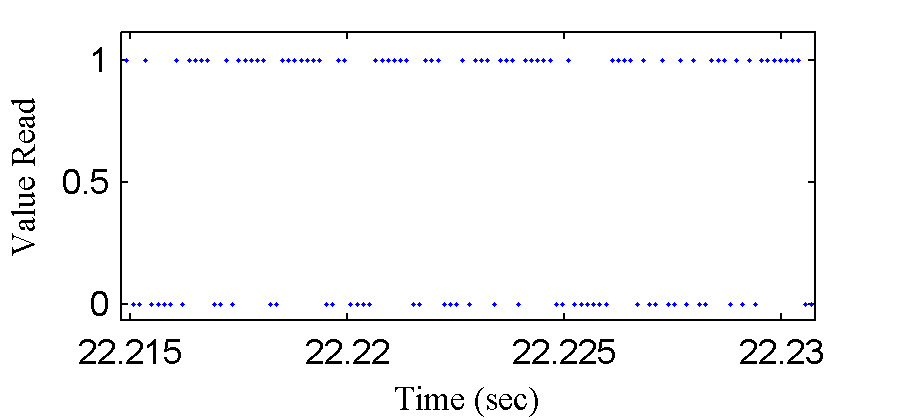
\includegraphics[width=\mywidth]{figs/thermal_noise.png} 
%\includegraphics[width=3.0in]{figs/eval_performance_diff_context.pdf} 
\caption{Thermal noise in Flash memory (time domain).}
\label{fig:thermal} 
\vspace{-0.25in}
\end{center} 
\end{figure} 

For Flash memory in practice, experiments show that two types of noise coexist: thermal noise and RTN. Thermal noise is white noise that exists in nearly all electronic devices. RTN can be observed only if a surface trap exists, the RTN amplitude is larger than that of thermal noise, and the sampling frequency (speed for continuous reads) is high enough. If any of these three conditions is not satisfied, only thermal noise will be observed as in Figure~\ref{fig:thermal}. In the case of thermal noise, a bit oscillates between the two states quickly, and the power spectral density (PSD) indicates white noise. 

\begin{figure}
  \centering
  \subfigure[][]{
    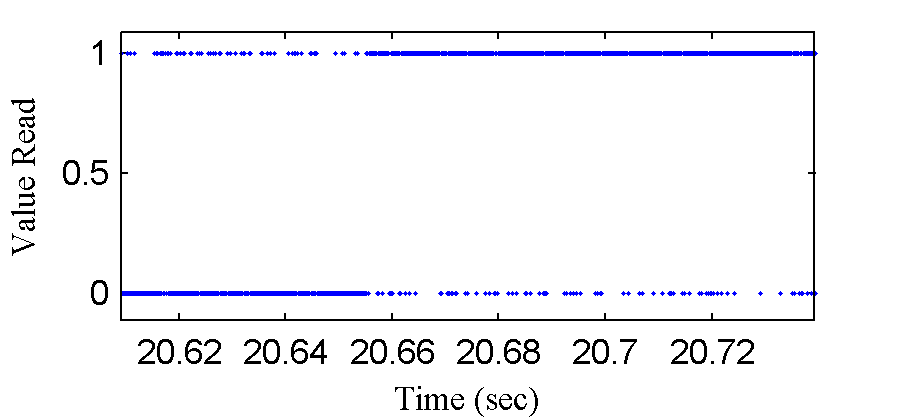
\includegraphics[width=\mywidth]{figs/thermal_rng_noise1.png}
    \label{fig:thermal_rtn1}
  }
  
  \subfigure[][]{
    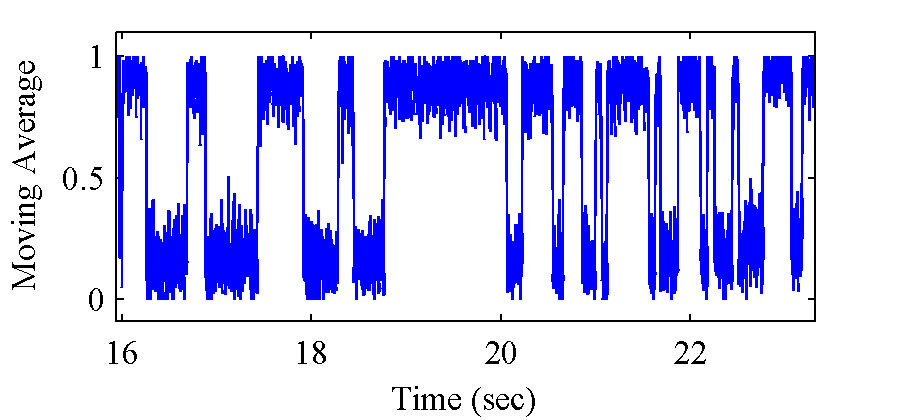
\includegraphics[width=\mywidth]{figs/thermal_rng_noise2.png}
    \label{fig:thermal_rtn2}
  }
  \caption{RTN with thermal noise in Flash memory. (a) Time domain. (b) Moving average of 29 points on the time domain.}
  \label{fig:thermal_rtn}
\end{figure}

In the case that the RTN amplitude is comparable to thermal noise, a combination of RTN and thermal noise is observed as shown in Figure~\ref{fig:thermal_rtn}. This is reflected by the density change of 1s in the continuous reading. A moving average on the time domain helps to visualize the density change. The PSD of the result shows $1/{f}^2$ spectrum at low frequencies and becomes flat at high frequencies.

\begin{figure} 
\begin{center} 
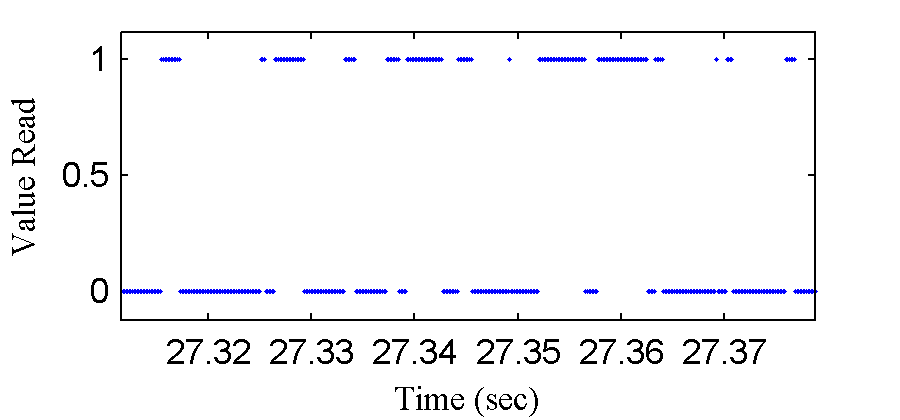
\includegraphics[width=\mywidth]{figs/rtn.png} 
%\includegraphics[width=3.0in]{figs/eval_performance_diff_context.pdf} 
\caption{RTN in Flash memory (time domain).}
\label{fig:rtn} 
\vspace{-0.25in}
\end{center} 
\end{figure} 

In some cases, the RTN amplitude is very high and dominates thermal noise. As a result, only RTN behaviors are visible through digital interfaces for these bits. As shown in Figure~\ref{fig:rtn}, continuous reads show clear clusters of 1s and 0s in the time domain. The power spectral density (PSD) of these bit sequences shows a clear RTN pattern of $1/{f}^2$. 

 
\begin{figure}
  \centering
  \subfigure[][]{
    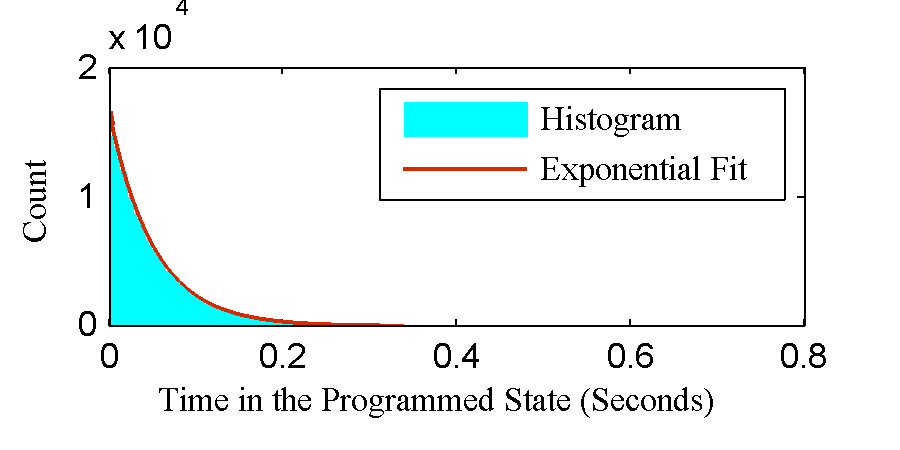
\includegraphics[width=\mywidth]{figs/rtn_freq_pstate.png}
    \label{fig:rtn_freq_pstate}
  }
  
  \subfigure[][]{
    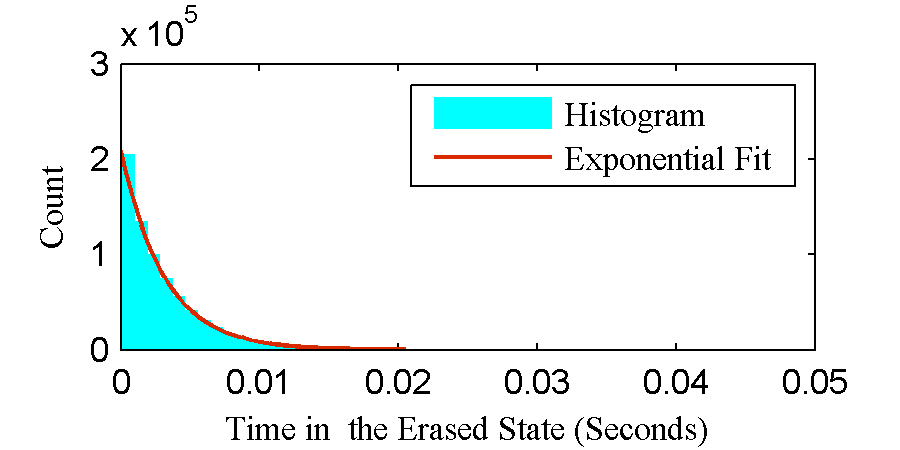
\includegraphics[width=\mywidth]{figs/rtn_freq_estate.png}
    \label{fig:rtn_freq_estate}
  }
  \caption{(a) Distribution of time in the programmed state. 
(b) Distribution of time in the erased state.}
  \label{fig:rtn_freq}
\end{figure}


For a bit with nearly pure RTN behavior, we further validated that the error pattern corresponds to RTN by plotting the distributions of up and down periods. As shown in Figure~\ref{fig:rtn_freq}, both up time and down time nicely fit an exponential distribution as expected. Overall, our experiments show that both RTN and thermal noise exist in Flash memory and can be observed through a digital interface. While both noise types can be used for random number generation, we focus on RTN, which is more robust to temperature changes.

\subsection{Random Number Generation Algorithms}

In Flash memory devices, RTN manifests as random switching between the erased state (consecutive 1s) and programmed state (consecutive 0s). At a high-level, our Flash random number generator (RNG) identifies bits with RTN behavior, either pure RTN or RTN combined with thermal noise, and uses a sequence of time in the erased state (called up-time) and the time in the programmed state (called down-time) from those bits. In order to produce random binary outputs, the RNG converts the up-time and down-time sequence into a binary number sequence, and applies the von Neumann extractor for de-biasing. We found that thermal noise itself is random and does not need to be filtered out.

\begin{figure} 
\begin{center} 

%\begin{scriptsize}
\begin{center}

\begin{tabular}{|c|}
\hline
\begin{minipage}[t]{3.2in}



\begin{tabbing}
{\bf Algorithm I  Overall Flash RNG algorithm }
\\
\\ Erase a block;
\\
\\ Num = 0;
\\ do \=
\\ \>Partially program a page for T;
\\ \>Num++;
\\
\\ \>Read Nbytes in a page N times, and record a 
\\ \>trace for each bit – trace[bit];
\\ \>{\bf For} \= each bit in Nbytes, not selected yet
\\ \>\>{\bf    If} \= (CheckRTN(trace[bit]) == true) 
\\ \>\>\>          Selected[bit] = yes;
\\ \>\>\>          NumProgram[bit] = Num;
\\ \>{\bf End for}
\\ \> repeat until most bits are programmed.
\\
\\ ProgramSelectBits(Selected);
\\
\\ Read selected bits M times, and record up-time and down-time;
\\ {\bf For} \= each bit
\\ \>      ConvertToBinary(rawdata);
\\ {\bf End for}


\end{tabbing}
\end{minipage}
\\ \hline
\end{tabular}
\end{center}
%\end{scriptsize}
 
\caption{Overall Flash RNG algorithm}
\label{fig:overal_rng_al} 
\vspace{-0.25in}
\end{center} 
\end{figure}

Algorithm I shows the overall RNG algorithm. To generate random numbers from RTN, the first step is to identify bits with RTN or both RTN and thermal noise. To do this, one block in Flash memory is erased and then multiple incomplete programs with the duration of T are applied. After each partial program, a part of the page is continuously read N times and the outcome is recorded for each bit. In our experiments, we chose to read the first 80 bits (10 bytes) in a page for 1,000 times. For each bit that has not been selected yet, the algorithm checks if RTN exists using CheckRTN() and marks the bit location if there is RTN. As an optimization, the algorithm also records the number of partial programs when a bit is selected. The algorithm repeats the process until all bits are checked for RTN. The second step is to partially program all of the selected bits to an appropriate level so that they will show RTN behavior. Finally, the algorithm reads the selected bits M times, records a sequence of up-time and down-time for each bit, and converts the raw data to a binary sequence. 

\begin{figure} 
\begin{center} 

%\begin{scriptsize}
\begin{center}

\begin{tabular}{|c|}
\hline
\begin{minipage}[t]{3.2in}



\begin{tabbing}
{\bf Algorithm II  Determine whether there is RTN in a bit }
\\
\\ {\bf If} \= trace[bit] has over 98\% 1/0s
\\ \>        {\bf Return} false;
\\ {\bf End if} 
\\
\\ Calculate the power spectrum density (PSD);
\\ Convert PSD to the log scale in both x-y;

\\ {\bf If} \= PSD slope is always $< T_{slope}$ for all high frequency ($> T_{freq}$)
\\ \> {\bf Return} RTN
\\ {\bf End if} 
\\
\\ {\bf If} \= PSD slope is $< T_{slope}$ at least one interval (Invl) at a high frequency ($> T_{freq}$)
\\ \> {\bf Return} RTN-Thermal
\\ {\bf End if}


\end{tabbing}
\end{minipage}
\\ \hline
\end{tabular}
\end{center}
%\end{scriptsize}
 
\caption{Determine whether there is RTN in a bit}
\label{fig:rtn_bit} 
\vspace{-0.25in}
\end{center} 
\end{figure}

The function CheckRTN() in Algorithm II determines whether there is RTN in a bit based on a trace from N reads. The algorithm first filters out bits that almost always (more than 98\%) produce one result, either 1 or 0. For the bits with enough noise, the algorithm uses the power spectral density (PSD) to distinguish RTN from thermal noise; PSD for RTN has a form of $1/{f}^2$ at a high frequency. To check this condition, the algorithm computes the PSD, and converts it to a log-scale in both x and y axes. If the result has a slope less than Tslope (we use -1.5, the ideal value is -2) for all frequencies higher than Tfreq (we use 200Hz), the algorithm categorizes the bit as RTN only. If the PSD has a slope less than Tslope for any interval larger than than Invl (we use 0.2) at a high frequency, the bit is categorized as a combination of RTN and thermal noise.

\begin{figure} 
\begin{center} 

%\begin{scriptsize}
\begin{center}

\begin{tabular}{|c|}
\hline
\begin{minipage}[t]{3.2in}



\begin{tabbing}
{\bf Algorithm III  Program selected bits to proper levels }
\\ {\bf where RTN could be observed. }
\\
\\ {\bf For} \= each selected bit
\\ \> Do (NumProgram[bit]-K) partial programs;
\\
\\ \> {\bf do} \= \{
\\ \>\>  Partially program the bit for T;
\\
\\ \>\>  Read the bit N times;
\\ \>\>  Find Max and Min for moving averages;
\\
\\ \>\> {\bf If} \= $Max > TMax$ and $Min < TMin$ 
\\ \>\>\>    Break;
\\ \>\> {\bf End if}
\\ \> \} repeat up to L times
\\ {\bf End for}


\end{tabbing}
\end{minipage}
\\ \hline
\end{tabular}
\end{center}
%\end{scriptsize}
 
\caption{Program selected bits to proper levels where RTN could be observed.}
\label{fig:prg_rtn} 
\vspace{-0.25in}
\end{center} 
\end{figure}

The function ProgramSelectBits() in Algorithm III programs selected bits to a proper level where RTN can be observed. Essentially, the algorithm aims to take each bit to the point near where they were identified to have RTN. The number of partial programs that were required to reach this point before were recorded in NumProgram[Bit]. For each selected bit, the algorithm first performs partial programs with the duration of T based on the number recorded earlier (NumProgram[Bit]-K). Then, the algorithm performs up to L more partial program operations until a bit shows RTN behavior. The RTN behavior is checked by reading the bit N times, and see if the maximum of moving averages is greater than a threshold ($TMax = 0.7$) and the minimum is less than another threshold ($TMin = 0.3$). 

\begin{figure} 
\begin{center} 

%\begin{scriptsize}
\begin{center}

\begin{tabular}{|c|}
\hline
\begin{minipage}[t]{3.2in}



\begin{tabbing}
{\bf Algorithm IV Convert the raw data to binary random sequence. }
\\
\\ {\bf If} \= the bit has both RTN and thermal noise
\\ \> {\bf For} \= each up/down-time in raw data
\\ \>\>   Output = LSB(up/down-time);
\\ \> {\bf End for}
\\ {\bf End if}
\\
\\ {\bf If} \= the bit has only RTN
\\ \> {\bf do} \= \{
\\ \>\> {\bf For} \= each up/down-time in raw data
\\ \>\>\>    Output = LSB(up/down-time);
\\ \>\>\>    Shift right up/down-time by one bit;
\\ \>\> {\bf End for}
\\ \> \} repeat until all up/down time are zero;
\\ {\bf End if}
\\
\\Perform von Neumann de-biasing


\end{tabbing}
\end{minipage}
\\ \hline
\end{tabular}
\end{center}
%\end{scriptsize}
 
\caption{Convert the raw data to binary random sequence.}
\label{fig:to_bin_seq} 
\vspace{-0.25in}
\end{center} 
\end{figure}

Finally, the function ConvertToBinary() converts the raw data to a binary random sequence. For bits with both RTN and thermal noise, the up-time and down-time tend to be short. So only the LSBs of these numbers are used. Essentially, for every up-time and down-time, the algorithm produces 1 if the time is odd and 0 otherwise. Effectively, this is an even-odd scheme. For bits with perfect RTN behavior, up-time and down-time tend to be longer and we use more LSBs from the recorded up/down-time. In this case, we first produce a bit based on the LSB, then the second LSB, the third LSB, and so on until all extracted bits become 0. Finally, for both methods, we apply the von Neumann de-biasing method. The method takes two bits at a time, throws away both bits if they are identical, and takes the first bit if different. This process is described in Algorithm IV.

The stability of the bits in the partially programmed state is also important. We define the stability as how long a bit stays in the partially programmed state where RTN behavior can be observed. This is determined by the retention time of the Flash memory chip and the amplitude of the RTN compared to the designed noise margin. Assume the amplitude of the RTN is Ar, the noise margin of Flash memory is An, and the Flash retention time is 10 year, then the stable time for random number generation after partial programming will be roughly $Ts=Ar/An*10$ years. This means that after time Ts, a bit needs to be reset and reprogrammed. In our experiments, the bit that is shown in Figure~\ref{fig:rtn_freq} was still showing ideal RTN behavior even after 12 hours.

\section{Experimental Results}

This section presents evaluation results for the random number generation techniques for Flash memory devices. The two main metrics for random number generation are randomness and throughput. For security, the RNG must be able to reliably generate true random numbers across a range of environmental conditions over time. For performance, higher throughput will be desirable. 

\subsection{Evaluation Setup}

\begin{figure}
\begin{center} 
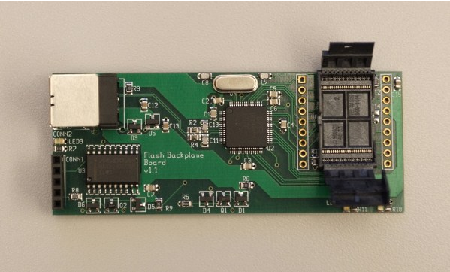
\includegraphics[width=\mywidth]{figs/flashtestboard.pdf} 
\caption{Flash test board.}
\label{fig:flashtestboard} 
\vspace{-0.1in}
\end{center} 
\end{figure} 

Our experiments use a custom Flash test board as shown in 
Figure~\ref{fig:flashtestboard}. The board is made entirely with 
commercial off-the-shelf (COTS) components with a custom PCB. 
There is a socket to hold a Flash chip under test, an ARM 
microprocessor to issue commands and receive data from the Flash 
chip, and a Maxim MAX-3233 chip to provide a serial (RS-232) 
interface. USB support is integrated into the ARM microcontroller. 
We also wrote the code to test the device. The setup represents 
typical small embedded platforms such as USB Flash drives, sensor 
nodes, etc. This device shows that the techniques can be applied 
to commercial off-the-shelf devices with no custom integrated 
circuits (ICs).

\begin{table}
  \begin{center}
    %\begin{scriptsize}
\begin{tabular}{|l|l|r|r|r|}
\hline

{\bf Manufacturer}& {\bf Part Number} & {\bf Size} & {\bf Qty} & {\bf Process} \\

\hline
Hynix & HY27UF084G2B & 4 Gbit & 10 & 5xnm class\\
       & & & & SLC\\
\hline
Micron & MT29F2G08ABA & 2 Gbit & 24 & 34nm \\
       & EAWP-IT:E4 & & & SLC\\
\hline
Micron & MT29F16G08CB & 16 Gbit & 5 & -- \\
       & ACAWP:C & & & MLC\\
\hline
Numonyx & NAND04GW & 4 Gbit & 3 & 57nm \\
& 3B2DN6 & & & SLC\\
 
\hline

\end{tabular}
%\end{scriptsize}
  \end{center}
\caption{Tested Flash chips.}
\vspace{-0.2in}
\label{tab:testedchips}
\end{table}

The experiments in this paper were performed with four types of Flash memory chips from Numonyx, Micron and Hynix, as shown in Table~\ref{tab:testedchips}.

\subsection{ Randomness}

Historically, three main randomness test suites exist. The first one is from Donald Knuth’s book “The Art of computer Programming (1st edition, 1969)” \cite{knuth1973art} which is the most quoted reference in statistical testing for RNGs in literature. Although it was a standard for many decades, it appears to be outdated in today’s view and it allows many “bad” generators to pass the tests. The second one is the “diehard” test suite from Florida State University. The test suite is stringent in the sense that they are difficult to pass. However, the suite has not been maintained in recent years. Therefore, it was not selected as the tests for this study. The third one is developed by National Institute of Standards and Technology (NIST) which is a measurement standard laboratory and a non-regulatory agency of the United States Department of Commerce. The NIST Statistical Test Suite is a package consisting of 15 tests that were developed to test the randomness of arbitrary long binary sequences produced by either hardware or software. The test suite makes use of both existing algorithms from past literatures and newly developed tests. The most updated version, sts-2.1.1, which was released in August 11, 2010, is used in our randomness tests. TABLE~\ref{tab:nist} summarizes the 15 NIST tests \cite{rukhin2001statistical}.

\begin{table}
  \begin{center}
    %\begin{scriptsize}
\begin{tabular}{|l|l|}
\hline

{\bf Test Name}& {\bf Test Description} \\

\hline
1 The Frequency & Tests proportion of zeros and \\
(Monobit) Test & ones for the whole sequence.\\
\hline
2 Frequency Test  & Tests the proportions of ones\\
within a Block    & within M-bit Block.\\
\hline
3 The Run Test & Tests the total number of runs in the \\
               & sequence, where a run is an uninterrupted \\
               & sequence of identical bits \\
\hline
4 Tests for the Longest- & Tests the longest run of ones within M-bit \\
Run-of-Ones in a Block & Block and consistency with theory \\
\hline
5 The Binary Matrix & Tests rank of disjoint sub-matrices \\
Rank Test & of the entire sequence and independence \\
\hline
6 The Discrete Fourier & Tests the peak heights in the Discrete Fourier  \\
Transform (Spectral) Test & Transform of the sequence, to detect periodic \\
                       & features that indicates deviation of randomness \\
\hline
7 The Non-overlapping & Tests the number of occurrences of\\
Template Matching Test & a pre-specified target strings \\
\hline
8 The Overlapping & Tests the number of occurrences of a \\
Template Matching Test & pre-specified target strings. When window \\
                   & found, slide only one bit before the next search \\
\hline
9 Maurer’s “Universal & Tests the number of bits \\
Statistics” Test & between matching patterns \\
\hline
10 The Linear & Tests the length of a linear feedback \\
Complexity Test & shift register, test complexity \\
\hline
11 The Serial Test & Tests the frequency of all \\
                  & possible overlapping m-bit pattern \\
\hline
12 The Approximate & Tests the frequency of all possible overlapping\\
Entropy Test &  m-bits pattern across the entire sequence \\
\hline
13 The Cumulative & Tests maximal excursion from the random walk \\
Sums (Cusums) Test & defined by the cumulative sum of adjusted \\
                  & (-1, +1) digits in the sequence \\
\hline
14 The Random & Tests the number of cycles having exactly K \\
Excursion Test & visits in a cumulative sum random walk \\
\hline
15 The Random Excursions & Tests the total number of times that a particular \\
Variant Test & state is visited in a cumulative sum random walk  \\

 
\hline

\end{tabular}
%\end{scriptsize}
  \end{center}
\caption{Summary of the NIST test suite}
\vspace{-0.2in}
\label{tab:nist}
\end{table}

Figure~\ref{fig:nist_result} shows one test result for the even-odd scheme, which only used an LSB from the up-time and down-time, when bits with both RTN and thermal noise are used. 10 sequences generated from multiple bits are tested and each sequence consists of 600,000 bits. Note that some of the results are not shown here due to the space constraint.  NonOverlappingTemplate, RandomExcursions and RandomExcursionsVariant have a lot of tests. In the result above, the proportion in the second column shows the proportion of the sequences which passed the test. If the proportion is greater than or equal to the threshold value specified at the bottom of the figure (8 out of 10 or 4 out of 5), then the data is considered random. The P-value in the first column indicates the uniformity of the P-values calculated in each test. If P-value is greater than or equal to 0.0001, the sequences can be considered to be uniformly distributed \cite{rukhin2001statistical}. The result indicates that the proposed RNG passes all the NIST tests. 

\begin{figure}
\begin{center} 
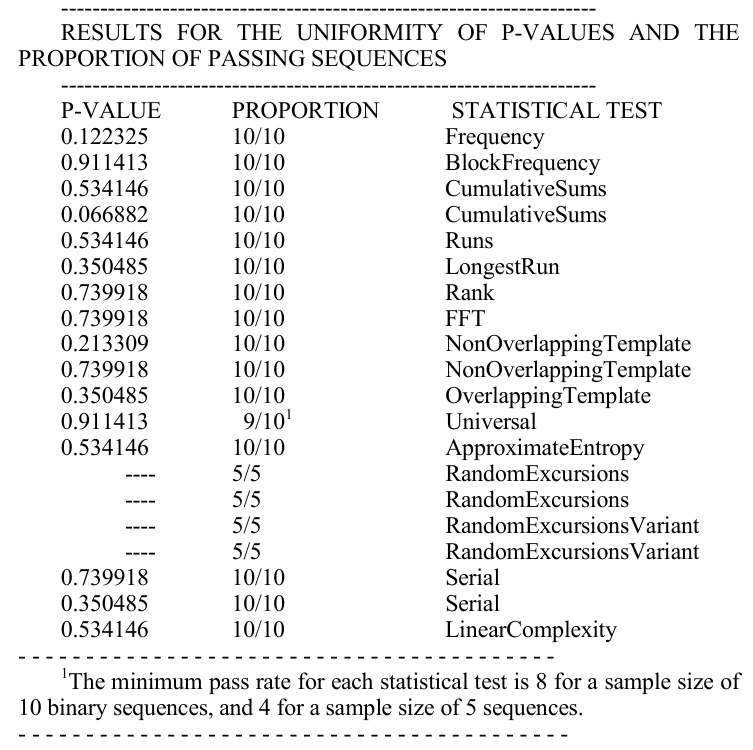
\includegraphics[width=5in]{figs/nist_result.png} 
\caption{NIST test suite results for bits with RTN and thermal noise.}
\label{fig:nist_result} 
\vspace{-0.1in}
\end{center} 
\end{figure} 

We also tested random numbers from one bit with only RTN behavior, using multiple bits from up-time and down-time. In this case, we generated ten 200,000-bit sequences from one bit. The data passed all NIST tests with results that are similar to the above case. For the Universal test, which requires a sequence longer than 387,840 bits, we used five 500,000-bit sequences. 

\subsection{Performance}

The throughput of the proposed RNG varies significantly depending on the switching rate of individual bits, sampling speed and environment conditions. Typically, only a small fraction of bits show pure RTN behavior with minimal thermal noise. TABLE~\ref{tab:pure_rtn} shows the performance of Flash chips from four manufacturers. The average throughput ranges from 848 bits/second to 3.37 Kbits/second. Note that the fastest switching trap that can be identified is limited by the reading speed in our experiments.


\begin{table}
  \begin{center}
    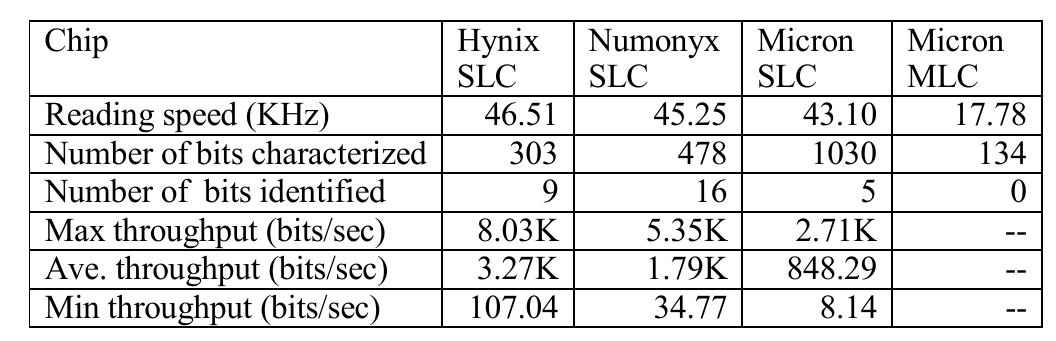
\includegraphics[width=5in]{figs/pure_rtn.png} 
  \end{center}
\caption{Performance of bits with pure RTN behavior.}
\vspace{-0.2in}
\label{tab:pure_rtn}
\end{table}

If bits with both RTN and thermal noise are also used, the percentage of bits which can be used for RNG can be much higher. The performance of these bits from the same Flash chips as in the pure RTN case is shown in TABLE~\ref{tab:rtn_and_thermal}. The average throughputs are higher because thermal noise is high frequency noise.

\begin{table}
  \begin{center}
    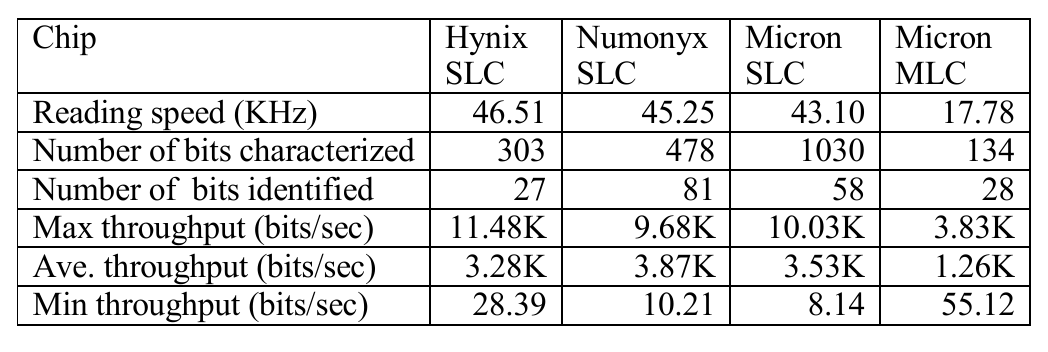
\includegraphics[width=5in]{figs/rtn_and_thermal.png} 
  \end{center}
\caption{Performance of bits with both RTN and thermal noise.}
\vspace{-0.2in}
\label{tab:rtn_and_thermal}
\end{table}

In our tests, the RNG throughput is largely limited by the timing of the asynchronous interface which is controlled by an ARM microcontroller with CPU frequency of 60MHz and the 8-bit bus for a Flash chip. We believe that the RNG performance can be much higher if data can be transferred more quickly through the interface. As an example, the average for RTN transition time is reported to range from 1 microsecond to 10 seconds \cite{abe2011understanding}. If a 128 bytes can be read in 6 microseconds which is the ideal random cache read speed for the Micron SLC chips, a RTN bit with 0.1ms average transition time will give approximately 20 Kbits/second throughput. Note that one page could have multiple RTN bits and our algorithm allows using multiple bits in parallel so that the aggregated throughput of an RNG can be much higher. For example, if N bits can be read at a time, in theory, that can increase the throughput by a factor of N. 

\subsection{Temperature Variations}

For traditional hardware RNGs, low temperatures present a particular challenge because thermal noise, which they typically rely on, can be reduced with the temperature. To study the effectiveness of the Flash-based RNG in low temperatures, we tested the scheme at two low temperature settings: one in a freezer, which is about -5°C, and the other in dry ice, which is about -80°C. The generated random sequences are tested individually as well as combined together with data from experiments at room temperature. All of them passed the NIST test suite without a problem, showing that our technique is effective at low temperatures.

Note that the experiments for temperature variations and aging are performed with a setup where data from Flash memory are transferred from a testbed to a PC through an USB interface. The post processing is performed on the PC. The USB interface limits the Flash read speed to 6.67KHz. As a result, the throughput in this setup is noticeably slower than the results in previous subsections where the entire RNG operation is performed on a microcontroller.  

To understand the impact of temperature variations on the Flash-based RNG, we tested the first 80 bits of a page from a Numonyx chip. At room temperature, 62 bits out of the 80 bits showed oscillations between the programmed state and erased state. 14 bits out of the 62 bits were selected by the selection algorithm, which identifies bits with pure RTN or both RTN and thermal components. The throughputs of the 14 bits are shown in Figure~\ref{fig:throughput_room_temp}. 

Figure~\ref{fig:throughput_m5_temp} and Figure~\ref{fig:throughput_m80_temp} show the performance of the RNG at -5 °C and -80 °C, respectively. At -5 °C, 79 bits out of 80 bits showed noisy behavior and 20 out of 79 bits were selected by the RNG algorithm as ones with RTN. At -80 °C, 72 bits out of 80 bits showed noise and 28 out of 72 bits were selected as the ones with RTN. On average, we found that per-bit throughput is slightly decreased at low temperatures, most likely because of reduced thermal noise and possibly because of slowed RTN switching. However, the difference is not significant. In fact, a previous study \cite{scofield2000temperature} claimed that RTN is temperature independent below 10 Kelvin. Interestingly, we found that the number of bits that are selected by our algorithm as ones with RTN behavior increases at a low temperature. This trend is likely to be because the low temperature decreases thermal noise amplitude while RTN amplitude stays almost the same and the RTN traps slow down so that they become observable at our sampling frequency. 

\begin{figure}
\begin{center} 
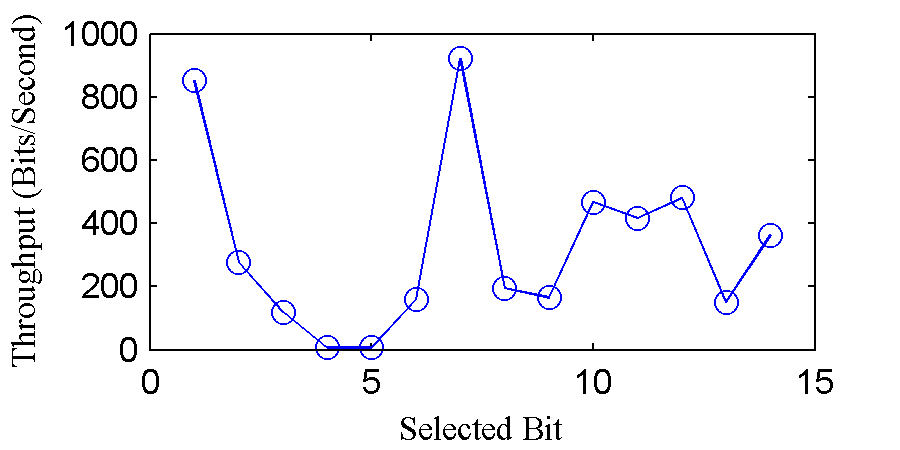
\includegraphics[width=\mywidth]{figs/throughput_room_temp.png} 
\caption{Throughputs under room temperature.}
\label{fig:throughput_room_temp} 
\vspace{-0.1in}
\end{center} 
\end{figure} 

\begin{figure}
\begin{center} 
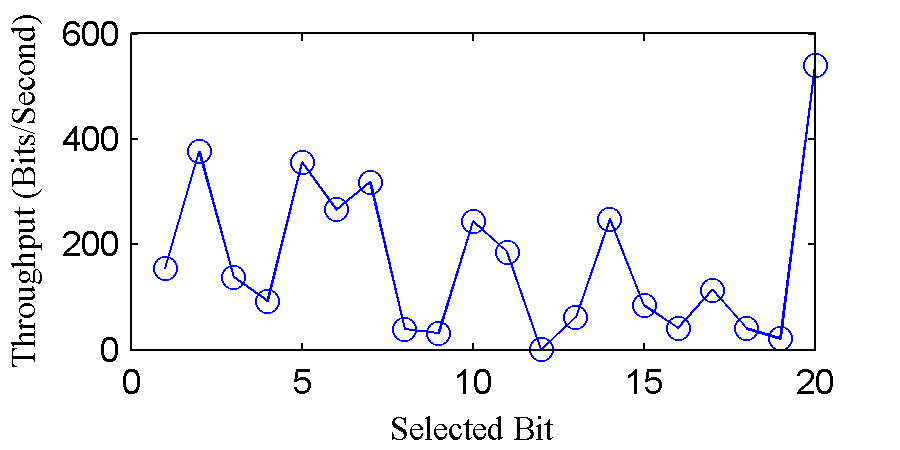
\includegraphics[width=\mywidth]{figs/throughput_m5_temp.png} 
\caption{Throughput at -5 °C.}
\label{fig:throughput_m5_temp} 
\vspace{-0.1in}
\end{center} 
\end{figure} 

\begin{figure}
\begin{center} 
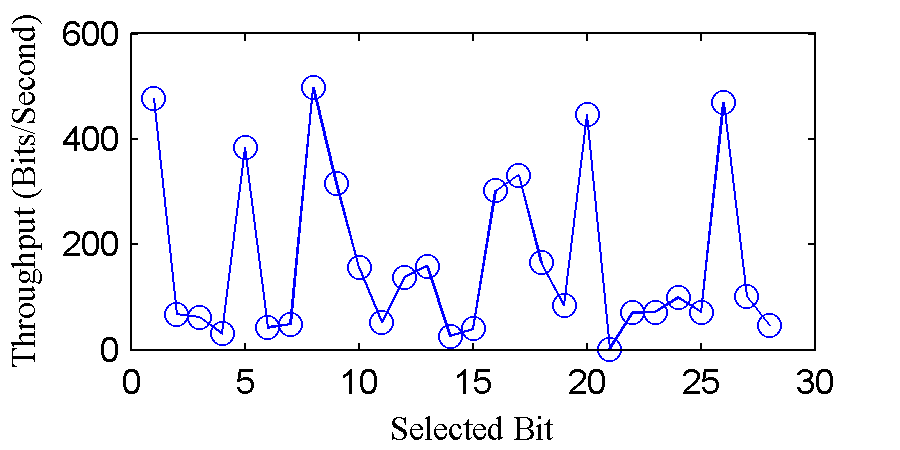
\includegraphics[width=\mywidth]{figs/throughput_m80_temp.png} 
\caption{Throughputs at -80 °C.}
\label{fig:throughput_m80_temp} 
\vspace{-0.1in}
\end{center} 
\end{figure} 

\subsection{Aging}

Flash devices wear-out over time as more program/erase (P/E) operations are performed. A typical SLC Flash chip has a lifetime of 1 million P/E cycles. In the context of RNGs, however, we do not think that wear-outs cause concerns. In fact, aging can create new RTN traps and increase the number of bits with RTN. To check the impact of aging on the RNG, we tested the scheme after 1,000 P/E operations and 10,000 P/E operations as shown in TABLE~\ref{tab:rtn_aging}. The RNG outputs passed the NIST test suite in both cases and did not show any degradation in performance. 

\begin{table}
  \begin{center}
    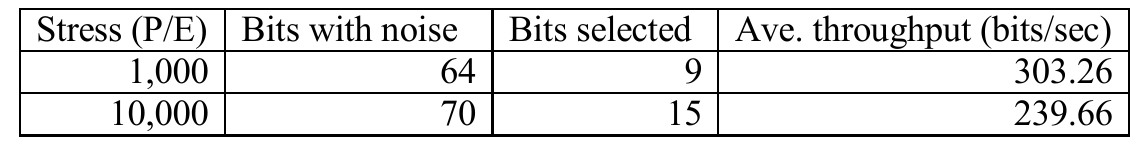
\includegraphics[width=5in]{figs/rtn_aging.png} 
  \end{center}
\caption{Performance summary of RTN in stressed pages}
\vspace{-0.2in}
\label{tab:rtn_aging}
\end{table}

The table shows an interesting trend that more bits show RTN behavior after 10,000 P/E cycles. The increase in noisy bits can potentially increase the overall RNG throughput. One possible concern with aging is a decrease in “stable time period” during which each bit shows noisy behavior. In our experiments, we found that a bit can be used for random number generation for over 12 hours after one programming (Algorithm III). If a bit is completely worn out, charge can leak out more quickly, requiring more frequent calibration. However, given that Flash memory is designed to have a retention time of 10 years within its lifetime, we do not expect the leakage to be a significant problem. We plan to perform larger scale experiments to understand how often a bit needs to be re-programmed for reliable random number generation. In practice, a check can also be added to ensure that a bit oscillates between 1 and 0. 

\section{Application Scenarios}

This section briefly discusses how the Flash memory based security functions, namely RNGs and device fingerprints, can be used to improve security of electronic devices. We first discuss where the techniques can be deployed and present a few use cases. 

The proposed Flash-based security techniques work with commercial off-the-shelf Flash memory chips using standard interfaces. For example, our prototype design is based on the Open NAND Flash Interface (ONFI) \cite{onfi}, which is used by many major Flash vendors including Intel, Hynix, Micron, and SanDisk. Other Flash vendors such as Samsung and Toshiba also use similar interfaces to their chips. 
The proposed techniques can be applied to any Flash or other floating-gate non-volatile memory, as long as one can control read, program (write), and erase operations to specific memory locations (pages and blocks), issue the RESET command and disable internal ECC. Embedded systems typically implement a Flash memory controller in software, exposing the low-level Flash chip interface to a software layer. Our prototype USB board in the evaluation section is an example of such a design. While we did not have a chance to study details, the manual for the TI OMAP processor family \cite{instruments2013omap}, which is widely used in mobile phones, indicates that its External Memory Interface (EMI) requires software to control each phase of NAND Flash accesses. In such platforms where Flash accesses are controlled by software, our techniques can be implemented as relatively simple software changes. 

For large memory components such as SSDs, the low-level interfaces to Flash memory chips may not be exposed to a system software layer. For example, SSD controllers often implement wear-leveling schemes that move data to a new location on writes. In such devices, the device vendor needs to either expose the Flash interfaces to higher level software or implement the security functions in firmware.  


The Flash-based random number generator (RNG) can either replace or complement software pseudo random number generators in any applications that need sources of randomness. For example, random numbers may be used as nonces in communication protocols to prevent replays or used to generate new cryptographic keys. Effectively, the Flash memory provides the benefits of hardware RNGs for systems without requiring custom RNG circuits. For example, with the proposed technique, low-cost embedded systems such as sensor network nodes can easily generate random numbers from Flash/EEPROM. Similarly, virtual machines on servers can obtain true random numbers even without hardware RNGs.

\section{Related Work}

Hardware random number generators generate random numbers from high-entropy sources in the physical world. Theoretically, some random physical processes are completely unpredictable. Therefore, hardware random number generators provide better random numbers in terms of randomness than software based pseudo-random number generators.

Thermal noise and other system level noise are the common entropy sources in recently proposed hardware random number generators. In \cite{sunar2007provably}, the phase noise of identical ring oscillators is used as the entropy source. In \cite{o2004puf}, the differences in path delays are used. In \cite{majzoobi2011fpga} and \cite{intelrng}, the metastability of flip-flops or two cross coupled inverters are used. Basically, the entropy source of these RNG designs is thermal noise and circuit operational conditions. These hardware random number generators can usually achieve high throughput because the frequency of the entropy sources is high. One common characteristic of these hardware random generators is that they all need carefully designed circuits where process variations should be minimized so that noises from the entropy source can be dominant. Compared to this, the random number generation in Flash memory cells does not require specially designed circuits and is more immune to process variation. Moreover, our entropy source is based on quantum behavior and theoretically, it should still work under extremely low temperatures where thermal noise or other kinds of noise decrease dramatically.


\chapter{Random Number Generation} \label{sec:fingerprints}

\section{Theory and Implementation}

This section describes techniques to generate unique fingerprints from Flash memory devices.

\subsection{Sources of Uniqueness}

Flash memory is subject to random process variation like any other semiconductor device. Because Flash is fabricated for maximum density, small variations can be significant. Process variation can cause each bit of a Flash memory to differ from its neighbors. While variation may affect many aspects of Flash cells, our fingerprinting technique exploits threshold voltage variations. Variations in doping, floating gate oxide thickness, and control-gate coupling ratio can cause the threshold voltage of each transistor to vary. Because of this threshold voltage variation, different Flash cells will need different times to be programmed.

\subsection{Extracting Fingerprints}

In this paper, we introduce a fingerprinting scheme based on partial programming. We repeatedly partially program a page on a Flash chip. After each partial program, some bits will have been programmed enough to flip their states from 1 to 0. For each bit in the page, we record the order in which the bit flipped. Pseudo-code is provided in Algorithm V. In our experiments, T is chosen to be 29.3us. A short partial program time provide a better resolution to distinguish different bits with the cost of increased fingerprinting time. We do not enforce all bits to be programmed, in order to account for the possibility of faulty bits.

\begin{figure} 
\begin{center} 

%\begin{scriptsize}
\begin{center}

\begin{tabular}{|c|}
\hline
\begin{minipage}[t]{3.2in}



\begin{tabbing}
{\bf Algorithm V  Extract the order in which bits in a page }
\\ {\bf reach the programmed state. }
\\
\\ Choose a partial programming time T (below the 
\\ rated program time). 
\\
\\ Nbits = number of bits in one page
\\ Order = 1; 
\\ Initialize BitRank[Nbits] to 0.
\\
\\ {\bf do} \= \{
\\ \>    Partially program a page for T;
\\ \>    {\bf For} \= all programmed bits {\bf do}
\\ \>\>        BitRank[programmed bit] = Order;
\\ \>    {\bf End for}
\\ \>    Order = Order + 1;
\\ \} repeat until most (99\%) bits in the page are programmed 


\end{tabbing}
\end{minipage}
\\ \hline
\end{tabular}
\end{center}
%\end{scriptsize}
 
\caption{Extract the order in which bits in a page reach the programmed state.}
\label{fig:extract_order} 
\vspace{-0.25in}
\end{center} 
\end{figure}

\subsection{Comparing Fingerprints}

The fingerprints extracted from the same page on the same chip over time are noisy but highly correlated. To compare fingerprints extracted from the same page/chip and different pages/chips, we use the Pearson correlation coefficient \cite{trust2011}, which is defined as

\begin{equation}
P(x,y)=\frac{E[(X-\mu_X)(Y-\mu_Y)]}{\sigma_X\sigma_Y}
\end{equation}

where X is the vector of program orders extracted from one experiment and Y is another vector of program orders extracted from another experiment. $\mu_X$ and $\sigma_X$ are the mean and standard deviation of the X vector. $\mu_Y$ and $\sigma_Y$ are the mean and standard deviation of the Y vector. 

In this way, the vector of program orders is treated as a vector of realizations of a random variable. For vectors extracted from the same page, $Y=aX+b+noise$ where a and b are constants and the noise is small. So, X and Y are highly correlated and the correlation coefficient should be close to 1. For vectors extracted from different pages, X and Y should be nearly independent of each other, so the correlation coefficient should be close to zero. From another perspective, if both X[i] and Y[i] are smaller or bigger than their means, $(X[i]-\mu_X)(Y[i]-\mu_Y)$ would be a positive number. If not, it would be a negative number. If X and Y are independent, it is equally likely to be positive and negative so the correlation coefficient would approach 0.

\begin{figure}
  \centering
  \subfigure[][]{
    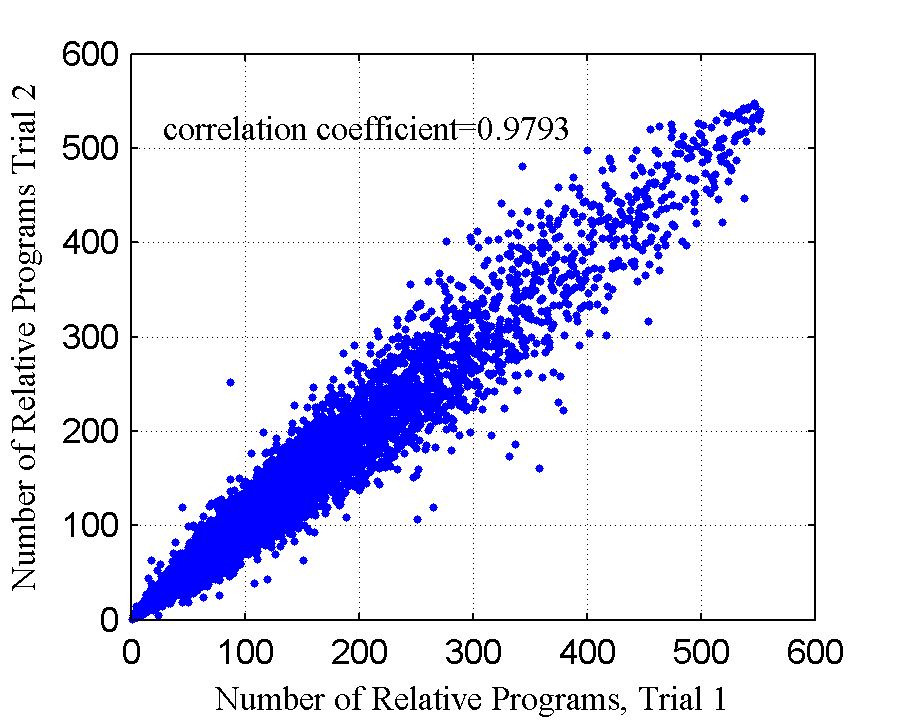
\includegraphics[width=\mywidth]{figs/fprints_same_page.png}
    \label{fig:fprints_same_page}
  }
  
  \subfigure[][]{
    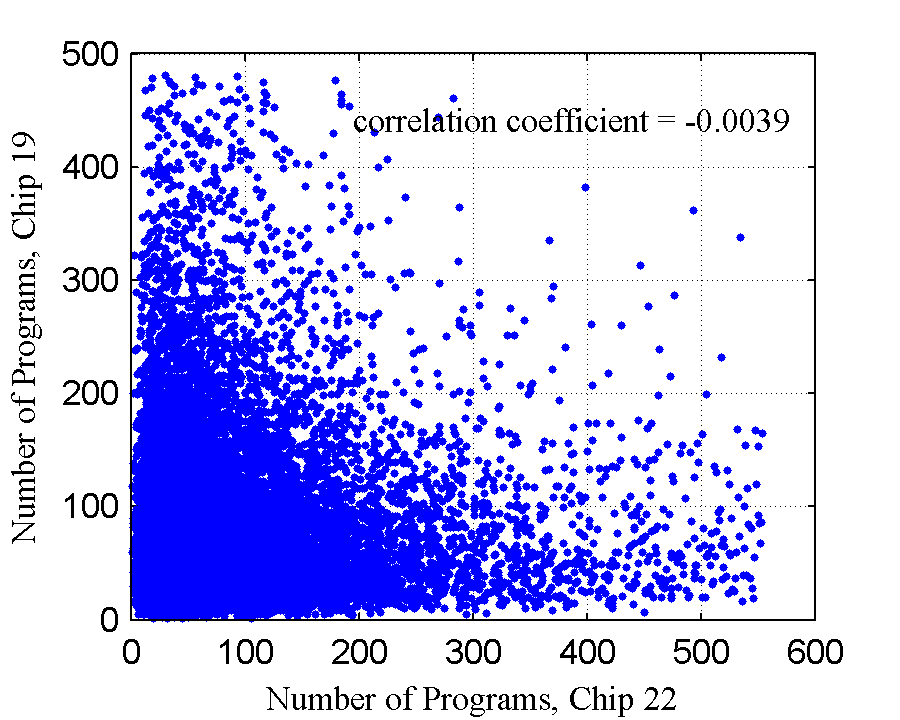
\includegraphics[width=\mywidth]{figs/fprints_diff_page.png}
    \label{fig:fprints_diff_page}
  }
  \caption{Scatter plot for fingerprints extracted on (a) the same page and (b) different chips.}
  \label{fig:fprints_scatter}
\end{figure}

The scatter plot of X and Y from the same page/chip and from different chips are shown in Figure~\ref{fig:fprints_scatter}. The figure clearly demonstrates a high correlation between fingerprints from the same chip over time and a low correlation between fingerprints from different chips. Therefore, this correlation metric can be used to compare fingerprints to determine whether they are from the same page/chip or from different pages/chips.

\subsection{Fingerprints in Binary Numbers}

The above fingerprints are in the form of the order in which each bit was programmed. If an application requires a binary number such as in generating cryptographic keys, we need to convert the recorded ordering into a binary number.

There are a couple of ways to generate unique and unpredictable binary numbers from the Flash fingerprints. First, we can use a threshold to convert a fingerprint based on the programming order into a binary number as shown in Algorithm VI. In the algorithm, we produce 1 if the program order is high, or 0 otherwise. This approach produces a 1 bit fingerprint for each Flash bit. Alternatively, we can obtain a similar binary fingerprint directly from Flash memory by partially programming (or erasing) a page and reading bits (1/0) from the Flash.

\begin{figure} 
\begin{center} 

%\begin{scriptsize}
\begin{center}

\begin{tabular}{|c|}
\hline
\begin{minipage}[t]{3.2in}



\begin{tabbing}
{\bf Algorithm VI  Generate a binary signature from the partial  }
\\ {\bf programming order information. }
\\
\\ Pick threshold $t = Max(BitRank) / 2$
\\ {\bf For} \= each bit
\\ \>    {\bf If} \= $BitRank[bit] > t$
\\ \>\>       Output 1
\\ \>    {\bf Else} Output 0
\\ {\bf End for}


\end{tabbing}
\end{minipage}
\\ \hline
\end{tabular}
\end{center}
%\end{scriptsize}
 
\caption{Generate a binary signature from the partial programming order information.}
\label{fig:gen_signature} 
\vspace{-0.25in}
\end{center} 
\end{figure}

\section{Evaluation}
 
The experiment setup and tested devices are the same as in the previous chapter. 

For fingerprinting, we are interested in uniqueness and robustness of fingerprints. The fingerprint should be unique, which means that fingerprints from different chips or different locations of the same chip must be significantly different – the correlation coefficient should be low. The fingerprint should also be robust, in a sense that fingerprints from a given location of a chip must stay stable over time and even under different environmental conditions – the correlation coefficient should be high.

In the experiments detailed below, we used 24 chips (Micron 34nm SLC), and 24 pages (6 pages in 4 blocks) from each chip. 10 measurements were made from each page. Each page has 16,384 bits.

\subsection{Uniqueness}

To test uniqueness, we compared the fingerprint of a page to the fingerprints of the same page on different chips, and recorded their correlation coefficients. A total of 66,240 pairs were compared – (24 chips choose 2) * 24 pages * 10 measurements. The results are shown in Figure~\ref{fig:fprints_histo_diff_chip}. The correlation coefficients are very low, with an average of 0.0076. A Gaussian distribution fits the data well, as shown in red.

\begin{figure}
\begin{center} 
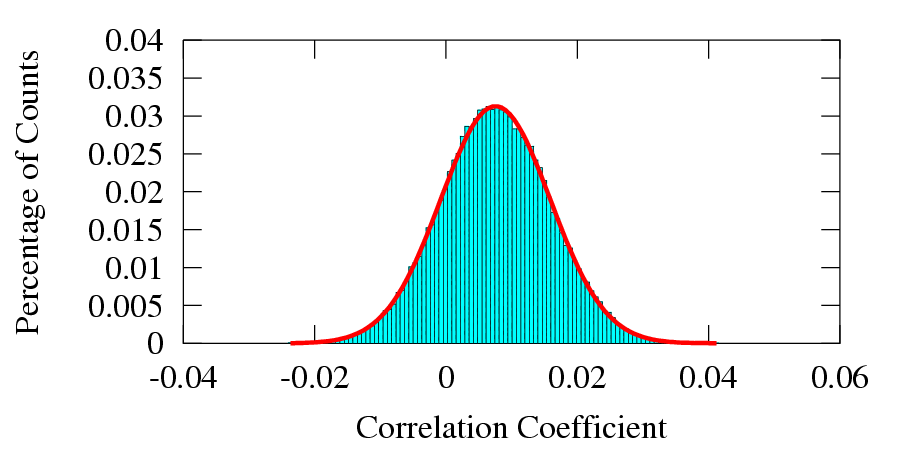
\includegraphics[width=\mywidth]{figs/fprints_histo_diff_chip.png} 
\caption{Histogram of correlation coefficients for pages compared to the same page on a different chip (total 66,240 comparisons).}
\label{fig:fprints_histo_diff_chip} 
\vspace{-0.1in}
\end{center} 
\end{figure} 

The correlation coefficients are also very low when a page is compared not only to the same page on different chips, but also to different pages on the same and different chips, shown in Figure~\ref{fig:fprints_histo_diff_page}. There are 1,656,000 pairs in comparison – ((24 pages * 24 chips) choose 2) * 10 measurements. This indicates that fingerprints from different parts (pages) of a chip can be considered as two different fingerprints and do not have much correlation. Therefore, the fingerprinting scheme allows the generation of many independent fingerprints from a single chip. The average correlation coefficient in this case is 0.0072.


\begin{figure}
\begin{center} 
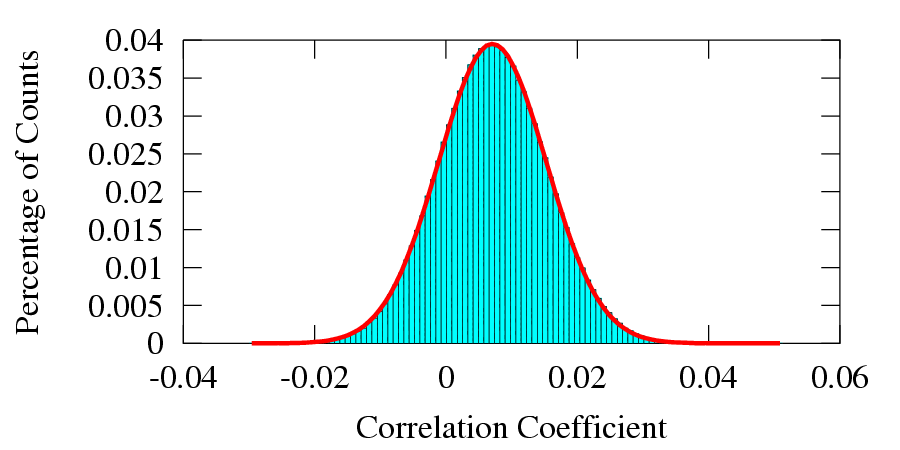
\includegraphics[width=\mywidth]{figs/fprints_histo_diff_page.png} 
\caption{Histogram of correlation coefficients for every page compared to every other page at room temp (total 1,656,000 comparisons).}
\label{fig:fprints_histo_diff_page} 
\vspace{-0.1in}
\end{center} 
\end{figure} 

\subsection{Robustness}

To test robustness, we compared each page’s measurement to the 9 other measurements of the same page’s fingerprint (an intra-chip measurement). The histogram of results for all pages is shown in Figure~\ref{fig:fprints_histo_same_page}. The correlation coefficient for fingerprints from the same page is very high, with an average of 0.9673. The minimum observed coefficient is 0.9022. The results show that fingerprints from the same page are robust over multiple measurements, and can be easily distinguished from fingerprints of a different chip or page. 

To be used in an authentication scheme, one could set a threshold correlation coefficient t. If, when comparing two fingerprints, their correlation coefficient is above t, then the two fingerprints are considered to have come from the same page/chip. If their correlation coefficient is below t, then the fingerprints are assumed to be from different pages/chips. 

\begin{figure}
\begin{center} 
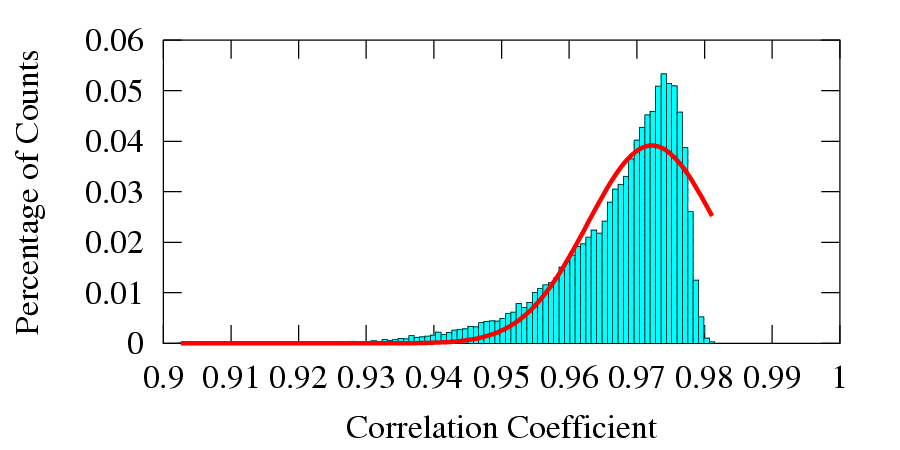
\includegraphics[width=\mywidth]{figs/fprints_histo_same_page.png} 
\caption{Histogram of correlation coefficients for all intra-chip comparisons (total 25,920 comparisons).}
\label{fig:fprints_histo_same_page} 
\vspace{-0.1in}
\end{center} 
\end{figure} 

In such a scheme, there is a potential concern for false positives and false negatives. A false negative is defined as comparing fingerprints that are actually from two different pages/chips, but deciding that the fingerprints are from the same page/chip. A false positive occurs when comparing fingerprints from the same page/chip, yet deciding that the fingerprints came from two different pages/chips. The threshold t can be selected to balance false negatives and positives. A high value of t would minimize false negatives, but increase the chance of false positives, and vice versa.

To estimate the chance of false positives and false negatives, we fit normal probability mass distribution functions to the correlation coefficient distribution. A false positive would arise from a comparison of two fingerprints from the same page being below t. The normal distribution fitted to the intra-chip comparison data in Figure~\ref{fig:fprints_histo_same_page} has an average $\mu = 0.9722$ and a std. deviation of 0.0095. For a threshold of $t = 0.5$, the normal distribution function estimates the cumulative probability of a pair of fingerprints having a correlation coefficient below 0.5 as $2.62*10^{539}$. At t = 0.7, the probability is estimated as $7.43*10^{-181}$.

The normal distribution function fitted to the inter-chip comparison data in Figure~\ref{fig:fprints_histo_diff_page} has a $\mu = 0.0076$ and a std. deviation of 0.0083. The estimated chance of a pair of fingerprints from different chips exceeding $t = 0.5$ is $4.52*10^{-815}$. At $t = 0.3$, the probability is estimated as $6.14*10^{-301}$.

The tight inter-chip and intra-chip correlations along with low probability estimates for false positives or negatives suggest that the size of fingerprints can possibly be reduced. Instead of using all 16,384 bits in a page, we can generate a fingerprint for a 1024-bit, 512-bit, or even only a 256-bit block. Experiments show that the averages of the observed correlation coefficients remain similar to those when using every bit in a page while the standard deviation increases by a factor of 2-3. However, the worst-case false negative estimates remain low. When using 256 bit fingerprints with the threshold $t = 0.3$, the estimate is $7.91*10^{-7}$. Under the same conditions, using 1024 bit fingerprints gives an estimated $3.20*10^{-22}$ chance of a false negative.

\subsection{Temperature Variations and Aging}

To see how robust the fingerprints are across different temperatures. We extracted fingerprints from chips at two other ambient temperatures, 60 °C and -5 °C. We tested a subset of the chips tested at room temperature – 6 pages (3 pages in 2 blocks) in 6 chips. 

Of interest is how fingerprints from the same page/chip, but taken at different temperatures, compare. Figure~\ref{fig:fprints_temp} shows the results of the intra-chip comparison between each temperature pair. Correlations remain high for fingerprints from the same page/chip, indicating that fingerprints taken at different temperatures can still be identified as the same. The average correlation coefficient is lower than when compared without a temperature difference, but is still sufficiently high to have very low false positive rates.

\begin{figure}
\begin{center} 
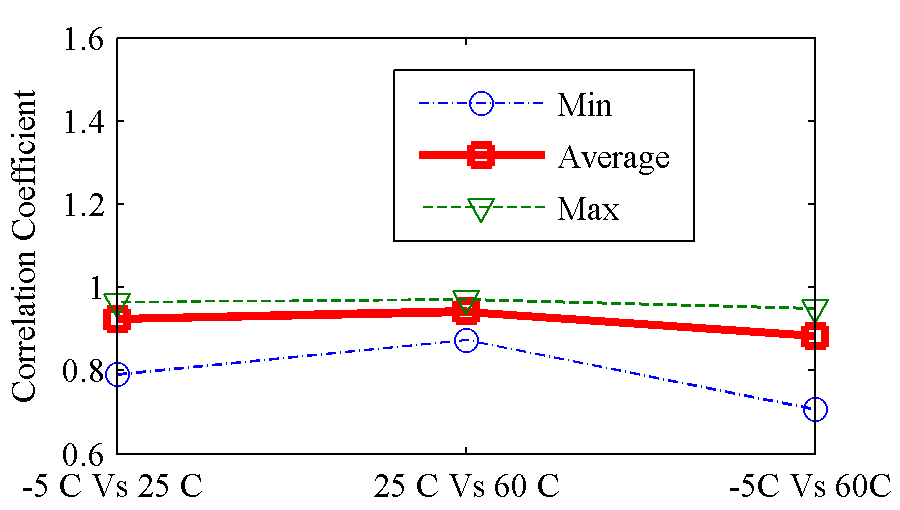
\includegraphics[width=\mywidth]{figs/fprints_temp.png} 
\caption{Average, minimum, and maximum correlation coefficients for intra-chip comparisons between different ambient temperatures.}
\label{fig:fprints_temp} 
\vspace{-0.1in}
\end{center} 
\end{figure} 

Comparing fingerprints from the same page at the same temperature at -5 °C or 60 °C still yields high correlation coefficients, as expected. Comparisons of fingerprints from different pages/chips at different temperatures give very low correlation coefficients.

\begin{figure}
\begin{center} 
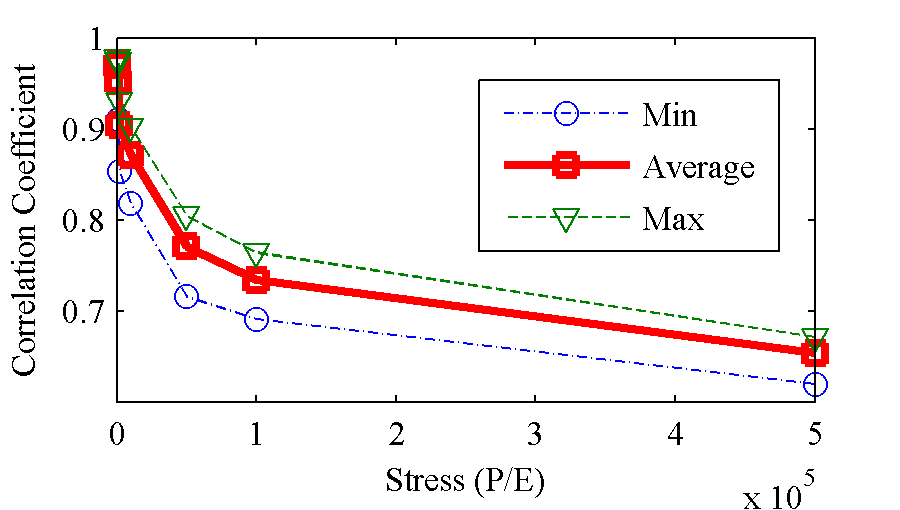
\includegraphics[width=\mywidth]{figs/fprints_aging.png} 
\caption{Average, minimum, and maximum correlation coefficients for comparisons between fresh and stressed Flash.}
\label{fig:fprints_aging} 
\vspace{-0.1in}
\end{center} 
\end{figure} 

Flash chips have a limited lifetime, wearing out over many program/erase (P/E) cycles. For a page’s fingerprint to be useful over time, fingerprints taken later in life should still give high correlation with younger fingerprints. Figure~\ref{fig:fprints_aging} shows the results of comparing fingerprints for the same page/chip taken when a Flash chip is new to fingerprints taken after a different number of P/E cycles. While the average correlation coefficient goes down noticeably, we note that it appears to bend towards an asymptote as the chip wears out. Even after 500,000 P/E cycles, which is beyond the typical lifetime of Flash chips, the average coefficient is still high enough to distinguish fingerprints of the same page/chip from fingerprints acquired from a different page/chip.

However, we found that an extreme wear-out such as 500,000 P/E cycles can raise a non-negligible false positive concern $(10^{-4})$ for short 256 or 512-bit fingerprints. This result indicates that we need longer fingerprints if they need to be used over a long period of time without a re-calibration.

\subsection{Security}

An attacker could attempt to store the fingerprints of a Flash device and replay the fingerprint to convince a verifier that he has the Flash chip in question. If the attacker cannot predict which page(s) or parts of a page (for shorter signatures) will be fingerprinted, he would need to store the fingerprints for every page to ensure success. The Flash chips in our experiments required about 800 partial program cycles per fingerprint. As the fingerprint comprises the order in which the bit was programmed, each bit’s ordering could be stored as a 10-bit number. To store an entire chip’s fingerprints would require 10x the chip storage. 

Acquiring a single fingerprint is relatively fast. Our setup could record an entire page’s fingerprint in about 10 seconds. However, there are 131,072 pages on our (relatively small) test chip; characterizing one chip would take about 2 weeks. The characterization time depends on the speed of the Flash interface, and we plan to further investigate the limit on how fast fingerprints can be characterized. 

\subsection{Applicability to Multiple Flash Chips}

Most of the above experimental results are obtained from the Micron SLC Flash memory. In order to answer the question of whether the proposed techniques are applicable to Flash memory in general, we have repeated both RNG and fingerprinting tests on four types of Flash memory chips in Table~\ref{tab:testedchips}, including an MLC chip.

The experiments showed that RNG and fingerprinting both work on all four types of Flash chips, with comparable performance. Detailed results are not included as they do not add new information. 

While we found that the proposed algorithm works without any change in most cases, there was one exception where the fingerprinting algorithm needed to be slightly modified in order to compensate for systematic variations for certain manufacturers. For example, for the Hynix and Numonyx chips, we found that bits from the even bytes of a page tend to be programmed quicker than bits from the odd bytes. Similarly, for the MLC chip, bits in a page divide into two groups: a quickly programmed group and a slowly programmed group. To accommodate such systematic behaviors, the fingerprinting algorithm was changed to only compare programming ordering of bits within the same group. 

\section{Application Scenarios}

One application of the Flash device fingerprints is to identify and/or authenticate hardware devices themselves similar to the way that we use biometrics to identify humans.

As an example, let us consider distinguishing genuine Flash memory chips from counterfeits through an untrusted supply chain. Recent articles report multiple incidents of counterfeit Flash devices in practice, such as chips from low-end manufacturers, defective chips, and ones harvested from thrown-away electronics, etc. \cite{trust2011, eetimesfakeparts, sosfakeflash}. The counterfeit chips cause a serious concern for consumers in terms of reliability as well as security; counterfeits may contain malicious functions. Counterfeits also damage the brand name for a manufacturer.

The Flash fingerprints can enable authentication of genuine chips without any additional hardware modifications to today’s Flash chips. In a simple protocol, a Flash manufacturer can put an identifier (ID) to a genuine chip (write to a location in Flash memory), generate a fingerprint from the chip, and store the fingerprint in a database along with the ID. To check the authenticity of a Flash chip from a supply chain, a customer can regenerate a fingerprint and query the manufacturer’s database to see if it matches the saved fingerprint. 

In order to pass the check, a counterfeit chip needs to produce the same fingerprint as a genuine one. Interestingly, unlike simple identifiers and keys stored in memory, device fingerprints based on random manufacturing variations cannot be controlled even when a desired fingerprint is known. For example, even legitimate Flash manufacturers cannot precisely control individual transistor threshold voltages, which we use to generate fingerprints. To produce specific fingerprints, one will need to create a custom chip that stores the fingerprints and emulates Flash responses.

The authentication scheme can be strengthened against emulation attacks by exploiting a large number of bits in Flash memory.  Figure~\ref{fig:auth_app} illustrates a modified protocol that utilizes a large number of fingerprints that can be generated from each Flash chip. Here, we consider a Flash chip as a function where a different set of bits that are used to generate a fingerprint is a challenge, and the resulting fingerprint is a response. A device manufacturer, when in possession of a genuine IC, applies randomly chosen challenges to obtain responses. Then, these challenge-response pairs (CRP) are stored in a database for future authentication operations. To check the authenticity of an IC later, a CRP that has been previously recorded but has never been used for a check is selected from the database, and a re-generated response from a device can be checked.

\begin{figure}
\begin{center} 
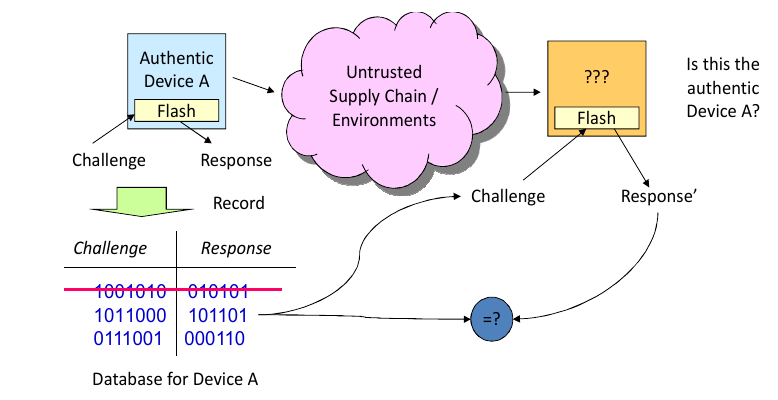
\includegraphics[width=\mywidth]{figs/authentication_app.png} 
\caption{Device authentication through a challenge-response protocol.}
\label{fig:auth_app} 
\vspace{-0.1in}
\end{center} 
\end{figure} 

Unless an adversary can predict which CRPs will be used for authentication, the adversary needs to measure all (or at least a large fraction) of possible fingerprints from an authentic Flash chip and store them in an emulator. In our prototype board, a generation of all fingerprints from a single page (16K bits) takes about 10 seconds and requires 10 bits of storage for each Flash bit. For a 16Gbit (2 GB) Flash chip, which is a moderate size by today’s standards, this implies that fully characterizing the chip will take hundreds of days and 20 GB storage. In the context of counterfeiting, such costs are likely to be high enough to make producing counterfeits economically unattractive. 

The security of the authentication scheme based on Flash fingerprints can be further improved if an additional control can be added to the Flash interface. For example, imagine using a USB Flash memory as a two-factor authentication token by updating its firmware to have a challenge-response interface for Flash fingerprints. Given that authentication operations only need to be infrequent, the USB stick can be configured to only allow a query every few seconds. If a fingerprint is based on 1024 Flash bits, fully characterizing an 8 GB USB stick can take tens of years.

In addition to device identification and authentication, the Flash fingerprints can be used as a way to produce many independent secret keys without additional storage. In effect, the proposed Flash fingerprints provide unpredictable and persistent numbers for each device. Previous studies such as fuzzy extractors \cite{dodis2004fuzzy} and Physical Unclonable Functions (PUFs) \cite{suhpuf2007} have shown how symmetric keys (uniformly distributed random numbers) can be obtained from biometric data or IC signatures from manufacturing variations by applying hashing and error correction. The same approach can be applied to Flash fingerprints in order to generate reliable cryptographic keys. A typical Flash with a few GB can potentially produce tens of millions of 128-bit symmetric keys.

\section{Related Work}

Instead of conventional authentication based on a secret key and cryptographic computation, researchers have recently proposed to use the inherent variation in physical characteristics of a hardware device for identification and authentication. Process variation in semiconductor foundries is a common source of hardware uniqueness which is out of the control of the designer \cite{boning1996statistical, bowman2002impact, nassif2000modeling}. A unique fingerprint can be extracted and used to identify the chip, but cannot be used for security applications because it can be simply stored and replayed. We also take advantage of process variation for our fingerprinting scheme. 
For security applications, Physical Unclonable Functions (PUFs) have been proposed. A PUF can generate many fingerprints per device by using complex physical systems whose analog characteristics cannot be perfectly replicated. Pappu initially proposed PUFs \cite{ravikanth2001physical} using light scattering patterns of optically transparent tokens. In silicon, researchers have constructed circuits which, due to random process variation, emit unique outputs per device. Some silicon PUFs use ring oscillators \cite{gassend2002silicon} or race conditions between two identical delay paths \cite{lee2004technique}. These PUFs are usually implemented as custom circuits on the chip. Recently, PUFs have been implemented without additional circuitry by exploiting metastable elements such as SRAM cells, which have unique value on start-up for each IC instance \cite{koeberl2011practical, holcomb2007initial}, or in Flash memories \cite{trust2011}. 
Our authentication scheme requires no new circuitry and can be done with commercially available and ubiquitous Flash chips. Unlike metastable elements, authentication does not require a power cycle. The scheme can generate many fingerprints by using more pages in the Flash chip. Acquiring a fingerprint is also faster and more widely applicable than previous Flash authentication methods.

\chapter{Hiding Information in Flash Memory} \label{sec:steg}

\section{Overview}
\label{sec:overview}

\subsection{Threat Model}

% Move to introduction.tex in order to place it on the 2nd page.
\begin{figure*} 
\begin{center} 
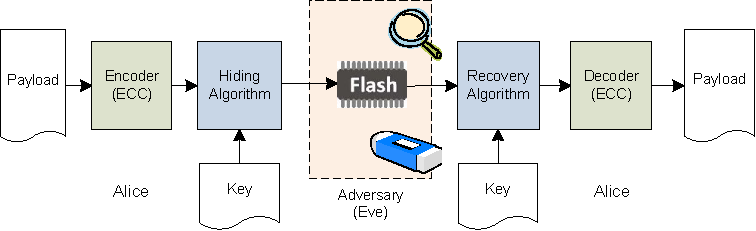
\includegraphics[width=6.5in]{figs/overview.pdf} 
%\includegraphics[width=3.0in]{figs/eval_performance_diff_context.pdf} 
\caption{The overview of the information hiding operation.}
\label{fig:overview} 
\end{center} 
\end{figure*} 

Figure~\ref{fig:overview} shows the overview of the information hiding
process in Flash memory. In order to hide information in Flash, Alice (left)
first adds an error correcting code (ECC) to her message payload and hides the
payload in the analog characteristics in Flash memory. Later, Alice (right) can
perform the reverse operations to retrieve the hidden payload by recovering
bits from the analog characteristics and correct errors using the ECC.
The information hiding and recovery algorithms use a secret key (hiding key)
%, often called {\em stego-key}, 
to determine where the hidden bits are stored in Flash memory. 
As error correcting codes are well studied, this paper focuses on the
physical encoding and decoding of information in Flash.

%As shown in the figure, the information hiding
%can be seen as a communication between two parties, from Bob (left) to
%Alice (right) in the figure \cite{simmons83}. 

As shown in the figure, an adversary (Eve) gets temporary access
to the Flash memory after Alice hides information. We assume that the adversary can inspect
and manipulate the memory through its normal interface, but do not consider physical
tampering of the memory. In the simple case, the adversary can check normal Flash operations
such as program, erase, and read operations. The adversary may also be aware of the information
hiding technique and can specifically check analog characteristics of Flash memory that
can be observed through the standard interface. 

The goal of the adversary may differ depending on the target application. In particular, the
adversary may try to
\begin{itemize}
\item Detect the existence of hidden information,
\item Retrieve the hidden information, or
\item Remove the hidden information.
\end{itemize}
For example, in the traditional steganography context where Alice is trying to establish 
a covert communication channel, it is important that the adversary cannot easily detect
the existence of hidden information. On the other hand, in the context of storing sensitive
information, it is more important that the adversary cannot retrieve information without
knowing the hiding key. For watermarking, it should be difficult to erase the hidden information.

Given an unlimited amount of time with the Flash chip, an adversary can break the information
hiding scheme by trying the retrieval algorithm on all pages with all possible hiding key values
because we assume that an adversary knows our hiding algorithm.
Therefore, the goal of the hiding technique is to make the detection, retrieval, and removal
of hidden information sufficiently time consuming for an attacker. 



%The proposed information hiding technique aims to enable reliable and
%secure communications. First, Bob should be able to reliably
%recover the hidden payload (in other words, the bit error rate after
%the recovery algorithm should be low enough to be corrected by the ECC).
%Second, it should be difficult for Eve to check whether there is
%hidden information or not, or recover the hidden information without
%the stego-key.
%Third, it should be difficult to for Eve to remove the hidden information.

%In this paper, we consider two types of adversaries. In the first case,
%an adversary is not aware of the proposed information hiding technique
%and only checks normal Flash operations and content. In this scenario,
%information hiding is successful if the hidden information cannot be found
%or removed by inspecting or erasing the Flash content. The proposed
%technique easily meets these conditions because hidden information is
%not encoded in the data stored in Flash memory.


%Interface - what is assumed about the interface. Abort function.
\subsection{Flash Interface Requirements}

The proposed technique is designed to work with Flash or other floating-gate 
non-volatile memory, as long as one can control read, program (write), and erase 
operations to specific memory locations (pages and blocks), issue the RESET 
command, and disable internal ECC (if there is any). 
For example, our experiments use off-the-shelf Flash chips that
use the Open NAND Flash Interface (ONFI) \cite{onfi}, which is used by 
many major Flash vendors including Intel, Hynix, Micron, and SanDisk. Other 
Flash vendors such as Samsung and Toshiba also use similar interfaces to their chips. 
In many embedded and mobile devices, the required interface functions are already
exposed to the software layers so that the proposed technique can be simply implemented
as a software update.

%Embedded systems typically implement a Flash memory controller in software, exposing the low-level Flash chip interface to a software layer. Our prototype USB board in the evaluation section is an example of such a design. While we did not have a chance to study details, the manual for the TI OMAP processor family \cite{instruments2013omap}, which is widely used in mobile phones, indicates that its External Memory Interface (EMI) requires software to control each phase of NAND Flash accesses. In such platforms where Flash accesses are controlled by software, our techniques can be implemented as relatively simple software changes. 



\section{Information Hiding Algorithm}
\label{sec:scheme}

This section describes the encoding (hiding) and decoding (recovery) algorithms 
for our information hiding scheme and the rationale for them. 

\subsection{Overview}

Our scheme hides information in the program time of
individual bits of Flash. The program time is the time it takes 
for a bit to change from the erased state (1) to the programmed state (0).
Normally, a Flash memory controller performs a program operation
at a page granularity, and the latency of this program operation is
determined by the slowest bit in a page to be successfully written.
In order to determine the program time for each bit, 
which we refer to as {\em per-bit program time}, we use the partial
programming technique that is described in the previous section.

\begin{figure} 
\begin{center} 
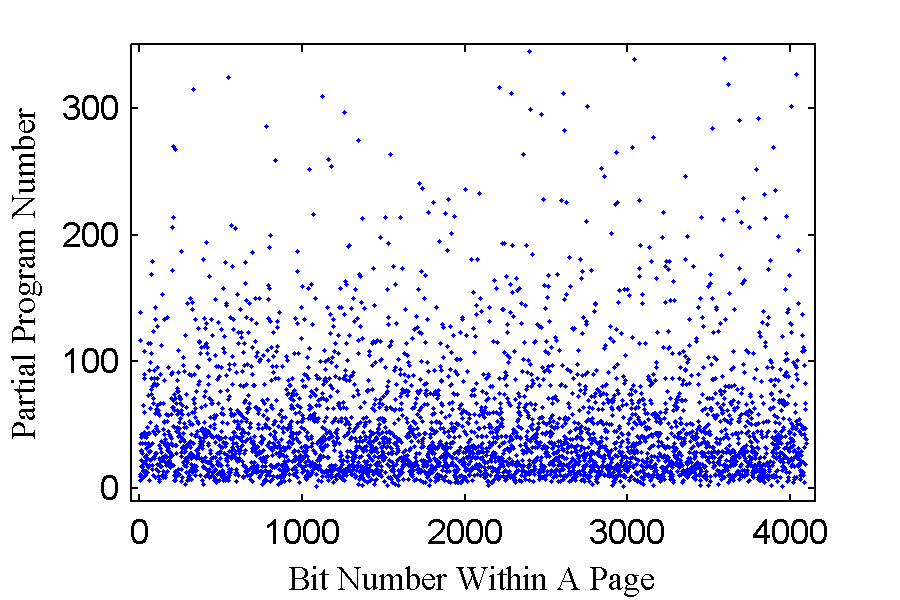
\includegraphics[width=\mywidth]{figs/program_numbers_c1_5e3pe_block1_page0.png} 
%\includegraphics[width=3.0in]{figs/eval_performance_diff_context.pdf} 
\caption{Raw partial program number for each bit in an example page.}
\vspace{-0.1in}
\label{fig:ptimeraw} 
\end{center} 
\end{figure} 

\begin{figure} 
\begin{center} 
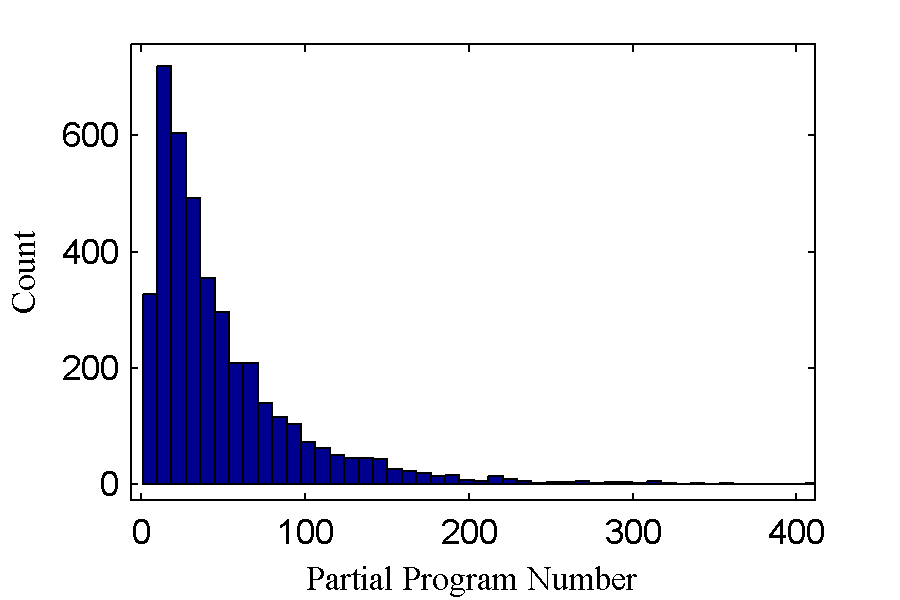
\includegraphics[width=\mywidth]{figs/hist_c1_block1_page1.png} 
%\includegraphics[width=3.0in]{figs/eval_performance_diff_context.pdf} 
\caption{Partial program time distribution for bits in a page.}
\vspace{-0.1in}
\label{fig:ptimehisto} 
\end{center} 
\end{figure} 

Figure~\ref{fig:ptimeraw} shows per-bit program times for a page. The plot
shows the number of partial program operations to flip state from 1 to 0 for each bit 
in a page. Because of process variations, the program time varies widely 
from bit to bit as shown in the figure. The per-bit program time distribution for the
page is shown in Figure~\ref{fig:ptimehisto}.
The wide distribution and noisy appearance of per-bit program times suggest that
small changes to each bit's program time would go unnoticed, and could be used to
carry a covert payload.

However, in order to hide information using the program time, we need to be able to 
intentionally change and control each bit's program time. Interestingly, in this
context, previous work has observed that program time tends to decrease as a Flash cell
becomes more worn-out \cite{grupp2009, trust2011}.
%varies depending on how worn-out a particular bit is
%A bit that is more worn-out shows a smaller program time.
In this work, we also found that how worn-out each bit is can be controlled
by selectively stressing a bit.
Although one can only program an entire page together, we can stress some bits
within a page more than others by controlling the value that we write.
During an erase operation, every bit
in a page is reset to an erased state (for example, assume that the erased state
represents '1').
On a program operation, only bits that switch to 0 experience
the program stress. When these bits are later erased, they also experience erase stress
as they are reverted to the 1 state. Therefore, bits that undergo
both switches (1 to 0 and 0 to 1) see the full program and erase stress
from one program and erase cycle. However, bits that store 1 will not be
switched to the 0 state by a program operation.
These bits see much less program and erase stress than their counterparts
which are programmed to 0 because their states do not need to change.
Therefore, by deciding whether to write a 1 or a 0 to each bit location 
in a page, we can control which bits are stressed more relative to 
other bits in the same page. 

In theory, if every bit had a similar program time without much variation,
we could hide one bit of information in every Flash bit by simply stressing or not
stressing the bit so that its program time encodes the hidden bit.
However, in practice, the program times of individual bits vary significantly
due to manufacturing variations, and intentional stress is often not sufficient 
to overcome the inherent variations; inherently slow bits will be likely to be
still slower than inherently fast bits even after being deliberately stressed.
To address this issue, we choose to encode 1 bit of hidden information %(stego-text)
using many bits in Flash memory. %(covertext). 
For each bit to hide, we choose a group of Flash bits and program them to the
same value, either 1 or 0. Effectively, this process encodes a bit in the collective
program time of the group. The averaging effect reduces variations among different
groups and allows the hidden bit to be more reliably recovered.

The use of a group also improves the security of the hiding scheme. In our scheme,
we use a key (hiding key) to select which Flash bits will be grouped together for
each hidden bit. If an attacker does not know the correct key, he or she cannot 
accurately identify which bits form a group together. 
Because an incorrect group is likely to contain both more stressed and less stressed
bits, the average program time of an incorrect group of bits will not show a clear
bias towards either 1 or 0. 

%Define "group" -- a group of bits in Flash that encode one bit of payload. This group
%is selected by a method known to the sender and receiver. We use a random selection
%of bits from the page to form a group.

\begin{figure} 
\begin{center} 
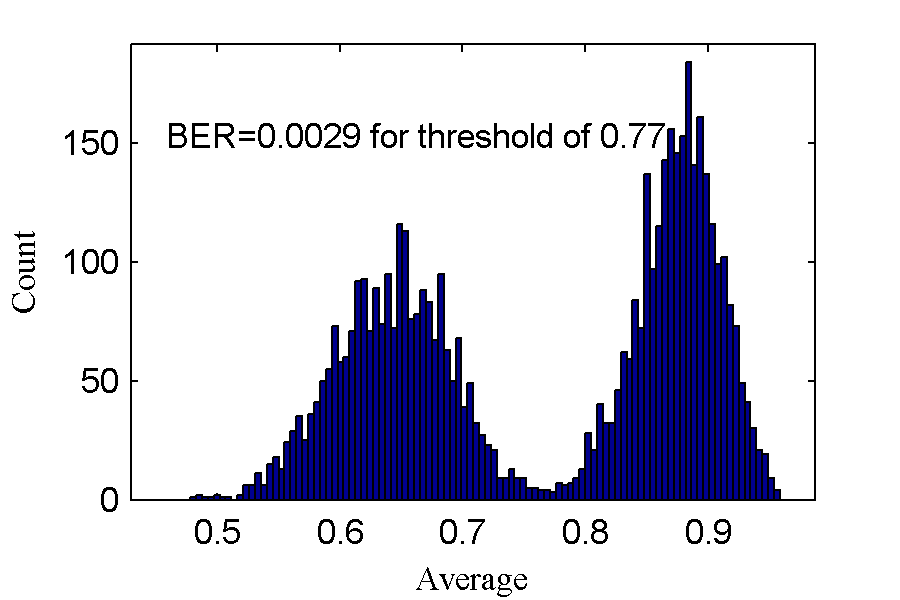
\includegraphics[width=\mywidth]{figs/5e3_histo_withkey.png} 
%\includegraphics[width=3.0in]{figs/eval_performance_diff_context.pdf} 
\caption{The distribution of the average program time of a group with a correct key.}
\label{fig:withkey_10blocks} 
\vspace{-0.1in}
\end{center} 
\end{figure} 

%To recover hidden information from the program time distribution,
%the intended recipient with the stego-key can compute the average
%program time for each group after the first thresholding. 
For example, Figure~\ref{fig:withkey_10blocks} shows the distribution of
the average program time of a correct group. In the experiment, we randomly selected
5,120 groups, each of which has 128 bits from a page, and hid either 1 or 0. 
As shown in the figure, these is an obvious gap in the distribution
between the fast and slow groups. Therefore, the value of hidden bits 
can be easily recovered through a simple thresholding. 
%We get a bit error rate (BER) of 0.0029 (0.29\%) in this case.
%even when a single
%quantization threshold ($X$) is used across all pages.


\begin{figure} 
\begin{center} 
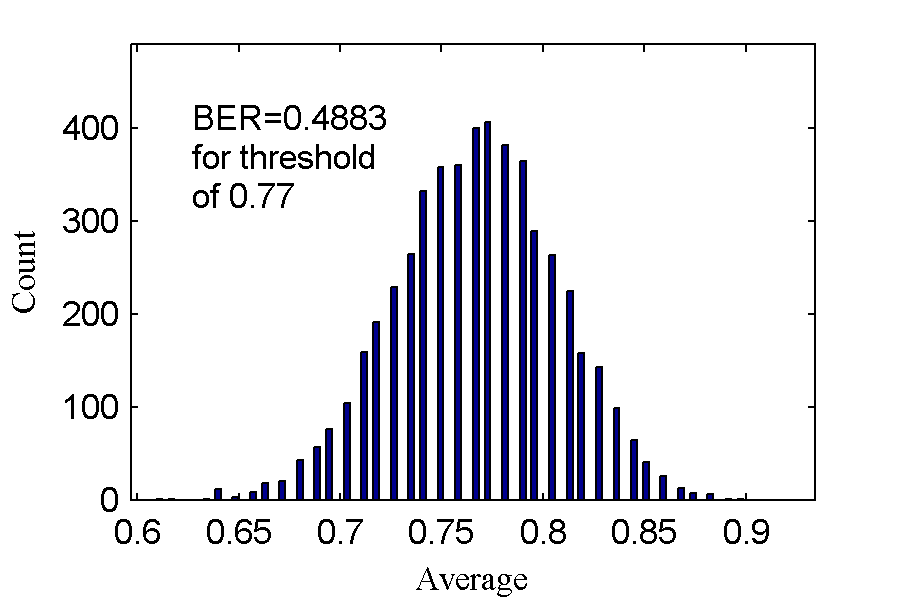
\includegraphics[width=\mywidth]{figs/5e3_histo_withoutkey.png} 
%\includegraphics[width=3.0in]{figs/eval_performance_diff_context.pdf} 
\caption{The distribution of the average program time of a incorrect group.}
\label{fig:withoutkey_10blocks} 
\vspace{-0.1in}
\end{center} 
\end{figure} 

On the other hand, Figure~\ref{fig:withoutkey_10blocks} shows the distribution
of the average program time when the hiding key is unknown. In this experiment,
we used a randomly selected hiding key. As shown in the figure, the average program
time of a group shows a normal distribution without any clear separation.
%The BER with the threshold $Th$ of 0.77 is 0.4883, which is close
%to 50\%. 
This result suggests that it is difficult for an adversary to recover hidden information 
without correct groupings because each group is likely to have both more and less
stressed bits.

%In fact, our experiments show that the distribution of individual bit's program
%time stays within a normal distribution even after the stress. As a result,
%it is difficult to tell whether any message is hidden within a page at all
%without knowing the correct key.



\subsection{Hiding Algorithm}

\begin{figure} 
\begin{center} 

%\begin{scriptsize}
\begin{center}

\begin{tabular}{|c|}
\hline
\begin{minipage}[t]{3.2in}



\begin{tabbing}
{\bf Algorithm I: Encoding }
\\
\\\emph{Part A -- Composing the message}
\\ 1 Fo\=r each selected page in a block
\\ 2 \>Generate the group for each message bit via the page hiding key
\\ 3 \>Assign each group 0 or 1 according to the embedded data
\\ 4 \>Fo\=r each bit
\\ 5 \>\>If\=\ its group will represent a message "1"
\\ 6 \>\>\>      Set it to be programmed 0
\\ 7 \>\>    Else
\\ 8 \>\>\>      Set it to be programmed 1
\\ 9 \>\>   End if
\\10 \>End for
\\11 End for
\\
\\\emph{Part B -- Writing the message to Flash}	
\\1 For each selected block
\\2 \>  For $i=1,2,..,N$ ($N$ is the number of Hiding PE cycles)
\\3 \>\>  Erase the block
\\4 \>\> Program every selected page
\\5 \>End for
\\6 End for


\end{tabbing}
\end{minipage}
\\ \hline
\end{tabular}
\end{center}
%\end{scriptsize}
 
\caption{An algorithm to encode (hide) a payload into Flash memory program time.}
\label{fig:encodingalg} 
\vspace{-0.25in}
\end{center} 
\end{figure}

Figure~\ref{fig:encodingalg} describes our methodology for hiding a payload in
program time of Flash memory. The algorithm is split into two parts: (A) composing the payload
by assigning bits of the message to groups of bits in Flash, and then (B) the actual process
of writing the payload to Flash by repeated program and erase stress.

For a given message, we first choose a set of pages and blocks in which to encode
the message based on the hiding key and the number bits that need to be hidden. 
Then, we divide the bits within each page into fixed size groups. % and record the groupings. 
Each group is used to store one message bit. 
The page, block, and group selections are based on the hiding key in a way that
cannot be predicted without the key. 
In our implementation, we used RC4 to choose the Flash bit locations for each message bit.

Then, the algorithm determines which value (0 or 1) needs to be written to each bit
location based on the message bit to be encoded.
If a group is to store a ``1'' value, we will
program (write a 0) the bits in the group, and the group will experience 
full program and erase stresses. If a group is to store a ``0'' value, the bits
in the group will be set to 1, and will see less stress.

With the payload mapped to bits in Flash memory, we perform the actual
write (program/erase) to Flash (Part B). We decide on a set number of stresses $N$ to exert
on the Flash. $N$ is chosen to ensure an acceptable
bit error rate without causing excessive stress. 
Each page is programmed $N$ times in order to imprint the
payload into the Flash.
In our experiments, we found that several hundred to a few thousand PE cycles are sufficient
for SLC chips. An even smaller amount of PE cycles are enough for MLC chips.


\subsection{Recovery Algorithm}

\begin{figure} 
\begin{center} 

\begin{footnotesize}
\begin{center}



\begin{tabular}{|c|}
\hline
\begin{minipage}[t]{3.2in}
\begin{tabbing}

{\bf Algorithm II: Decoding }
\\
\\\emph{Part A -- Reading the program time from Flash}
\\1 Fo\=r each selected block
\\2 \>Erase the block
\\3 \>Program every bit in the block to 0
\\4 \>Erase the block 
\\5 \>Fo\=r each selected page
\\6 \>\>Fo\=r $i=1,2, ..., M$  %(at least half of bits should flip after M iterations)
\\7 \>\>\>  Partial program the page to 0 (abort a program operation after time $T$)
\\8 \>\>\>  Read the page
\\9 \>\>\>  Fo\=r each bit in the page
\\10 \>\>\>\>If\=\ the bit changed from 1 to 0
\\11 \>\>\>\>\>   Set $program time$ for this bit to $i$
\\12 \>\>\>\>End if
\\13 \>\>\>End for
\\14 \>\>End for
\\15 \>\>Fo\=r each bit
\\16 \>\>\>If\=\ the bit did not flip
\\17 \>\>\>\>Set its $program time$ to be $M+1$ 
\\18 \>\>\>End if
\\19 \>\>End for
\\20 \>End for
\\21 \>Erase the block
\\22 End for
\\
\\\emph{Part B -- Extracting the payload message}
\\1 Fo\=r each selected block
\\2 \>Fo\=r each selected page
\\3 \>\>Calculate the median $X$ of the program times for all the bits
\\4 \>\>Fo\=r each bit
\\5 \>\>\>If its $programtime > (X/2)$
\\6 \>\>\>\>Set $program time$ to 1
\\7 \>\>\>Else
\\8 \>\>\>\>Set $program time$ to 0
\\9 \>\>\>End if
\\10 \>\>End for

\\11 \>\>Generate the group for each message bit with the page hiding key
\\12 \>\>For each group
\\13 \>\>\>Calculate the average program time for the group
\\14 \>\>\>If the average is less than $Th$
\\15 \>\>\>\>Recover the message bit: 1
\\16 \>\>\>Else
\\17 \>\>\>\>Recover the message bit: 0
\\18 \>\>\>End if
\\19 \>\>End for

%\\15 \>\>If the number of Hiding PE cycles $N < 2500$
%\\16 \>\>\>threshold $Th$ = fixed value $Th_f$
%\\17 \>\>Else
%\\18 \>\>\>sort the average program times
%\\19 \>\>\>find the maximum interval for the sorted program times
%\\20 \>\>\>threshold $Th$ = middle point of the maximum interval
%\\21 \>\>End if
%\\22 \>\>For each group
%\\28 \>\>End for

\\20 \>End for
\\21 End for
\end{tabbing}
\end{minipage}
\\ \hline
\end{tabular}
\end{center}
\end{footnotesize}
 
\caption{An algorithm to decode (recover) a payload from Flash memory program time.}
\label{fig:decodingalg} 
\vspace{-0.25in}
\end{center} 
\end{figure}


Figure~\ref{fig:decodingalg} describes our algorithm to decode a payload hidden 
by our encoding algorithm in Flash bit program time. Again, the algorithm is divided into
two parts: (A) physically reading the per-bit program time from Flash, and (B) recomposing
the payload from the program time distribution.

To read the hidden information, we must measure the program times for every bit in the pages
containing the hidden bits. To do so, we use the partial programming algorithm described 
in the previous section. We choose $M$ such that at the end of $M$ partial programs, 
more than half of the bits, are programmed.
% We used $M = 1200$ in our experiments. 
The program time of a bit is expressed as the number of partial program cycles needed to 
flip the bit from 1 to 0. 
For the bits that do not flip after the $M$ partial program operations, their program
times are set to be a constant above $M$ (i.e. $M+1$). 
%The length of a partial program
%($T$) is chosen to be small enough to be able to measure differences in program times.

To reconstruct the payload from the per-bit program times, we apply two thresholding steps. 
First, we compute the median program time $X$ across all bits within each page.
Then, the program time of each bit within a page is quantized based on the median;
if a bit's program time is above half the median
program time ($X/2$), then its program time is set to 1; otherwise it is set to 0.
%\textbf{TODO: HOW IS X/2 CHOSEN?}
($X/2$) was chosen empirically.

The bits are then divided into the groups specified by the hiding key. Within each group, 
the average of each individual bit's program times (now consisting of only 1 and 0) is 
computed, and the second thresholding step
is performed. Each bit in the payload is set to 1 if the average program time
of the corresponding group is below the threshold $Th$. Otherwise, the bit is set to 0.

In practice, with sufficient hiding PE cycles, we saw that there exists an obvious gap 
between the average program times of the more-stressed and less-stressed groups. 
As a result, it is straightforward to set the threshold $Th$ to distinguish the
two types of groups. For each page, we first sort the average program time of each
group. Suppose the sequence of sorted program times is $X0, X1, X2, ..., XN$. Then 
we calculate the intervals between the sorted average program times and get $X1-X0, X2-X1, ...$.
Suppose the maximum interval is $XM-XL$, then we set the threshold to be in the middle of that
interval; $Th = (XM+XL)/2$. In this way, we can get a per-page threshold. 
For the cases with low hiding PE cycles, where there is no clear gap between the two
clusters, the threshold is set to be a constant across pages based on the histogram
of the average program times from multiple blocks. 
 
%The threshold $Th$ is decided after plotting the averages. In practice,
%we saw that the groups would sort themselves into two clusters. Taking a histogram
%of the averages, we set the threshold $Th$ to be the lowest value in the gap between
%the two clusters.

For simplicity, we describe and evaluate the algorithm for the case where all bits 
within a selected page are used to hide bits. In order to make detection more
difficult, it is also possible to only use a small subset of bits within a page.
We leave this variant for future work.



\section{Evaluation}
\label{sec:evaluation}

In this section we evaluate the proposed scheme through experiments on 
Flash chips. In addition to validating correct operation of the 
encoding and decoding algorithms, we also study the robustness across 
various design parameters, performance, detectability, recovery 
without the hiding key, and erase tolerance.

\subsection{Evaluation Setup}

\subsubsection{Testbed Device}

\begin{figure}
\begin{center} 
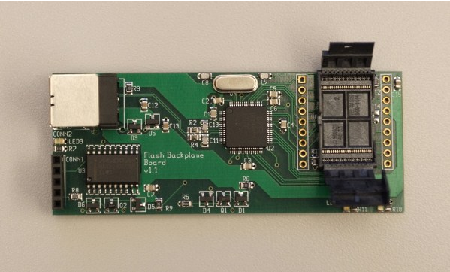
\includegraphics[width=\mywidth]{figs/flashtestboard.pdf} 
\caption{Flash test board.}
\label{fig:flashtestboard} 
\vspace{-0.1in}
\end{center} 
\end{figure} 

Our experiments use a custom Flash test board as shown in 
Figure~\ref{fig:flashtestboard}. The board is made entirely with 
commercial off-the-shelf (COTS) components with a custom PCB. 
There is a socket to hold a Flash chip under test, an ARM 
microprocessor to issue commands and receive data from the Flash 
chip, and a Maxim MAX-3233 chip to provide a serial (RS-232) 
interface. USB support is integrated into the ARM microcontroller. 
We also wrote the code to test the device. The setup represents 
typical small embedded platforms such as USB Flash drives, sensor 
nodes, etc. This device shows that the techniques can be applied 
to commercial off-the-shelf devices with no custom integrated 
circuits (ICs).

\subsubsection{Flash Memory Chips}

\begin{table}
  \begin{center}
    %\begin{scriptsize}
\begin{tabular}{|l|l|r|r|r|}
\hline

{\bf Manufacturer}& {\bf Part Number} & {\bf Size} & {\bf Qty} & {\bf Process} \\

\hline
Hynix & HY27UF084G2B & 4 Gbit & 1 & 5xnm class\\
       & & & & SLC\\
\hline
Micron & MT29F2G08ABA & 2 Gbit & 5 & 34nm \\
       & EAWP-IT:E4 & & & SLC\\
\hline
Micron & MT29F4G08ABA & 4 Gbit & 15 & 34nm \\
       & DAWP:D & & & SLC\\
\hline
Micron & MT29F16G08CB & 16 Gbit & 1 & -- \\
       & ACAWP:C & & & MLC\\
\hline
Numonyx & NAND04GW & 4 Gbit & 1 & 57nm \\
& 3B2DN6 & & & SLC\\
 
\hline

\end{tabular}
%\end{scriptsize}


  \end{center}
\caption{Tested Flash chips.}
\vspace{-0.2in}
\label{tab:testedchips}
\end{table}

The experiments in this paper were performed with five types of 
Flash memory chips from Numonyx, Micron, and Hynix. 
Table~\ref{tab:testedchips} shows their details. 
We primarily performed experiments with Micron 4Gbit chips.
Experiments using other models will be marked.

In most experiments, we only used the first 4,096 bits of 16,896-bit pages to
avoid performance overheads given the limited amount of memory in the microcontroller.
We will refer to the first 4,096 bits as a ``page'' in the following discussion.
For the analyses of per-page read/program time and per-block erase time, we
used the entire page.


%\subsection{Overall Operation}

%WE MAY REMOVE THIS SUBSECTION.

%\begin{figure} 
%\begin{center} 
%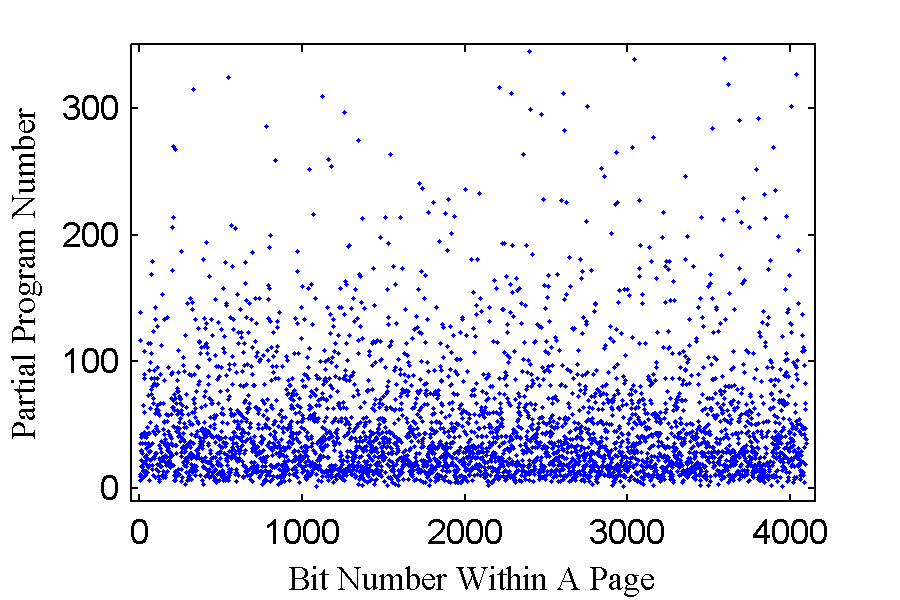
\includegraphics[width=\mywidth]{figs/program_numbers_c1_5e3pe_block1_page0.png} 
%%\includegraphics[width=3.0in]{figs/eval_performance_diff_context.pdf} 
%\caption{Raw partial program numbers for bits in a page.}
%\vspace{-0.1in}
%\label{fig:ptimeraw} 

%\end{center} 
%\end{figure} 


%\begin{figure} 
%\begin{center} 
%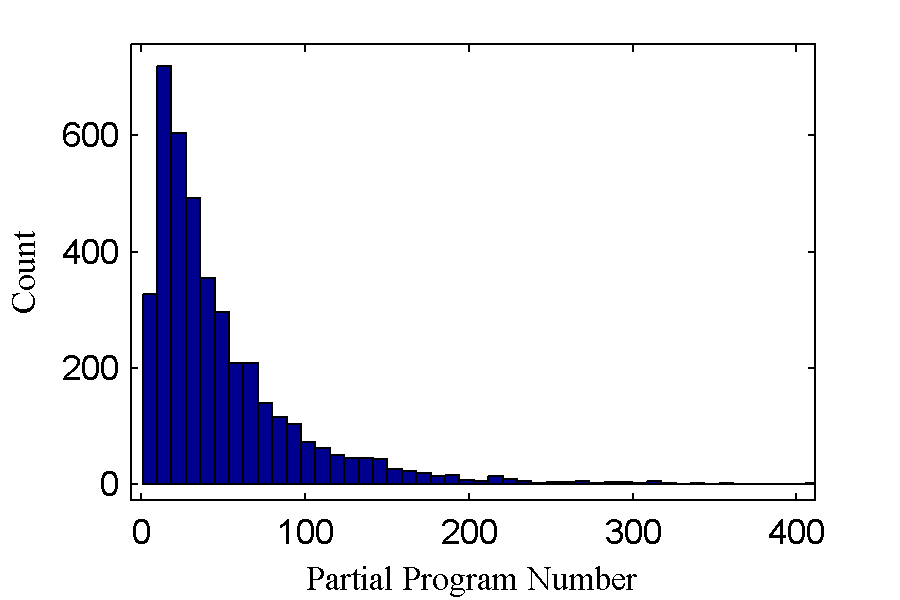
\includegraphics[width=\mywidth]{figs/hist_c1_block1_page1.png} 
%%\includegraphics[width=3.0in]{figs/eval_performance_diff_context.pdf} 
%\caption{Partial program time distribution for bits in a page.}
%\vspace{-0.1in}
%\label{fig:ptimehisto} 

%\end{center} 
%\end{figure} 

%Figure~\ref{fig:ptimeraw} shows the raw program numbers for the 
%bits in a page with hidden information. The program time distribution 
%is shown in Figure~\ref{fig:ptimehisto}. The first 4,096 bits of the 
%page are used and 
%they are divided into 32 groups randomly based on the stego-key.
%5,000 program and erase cycles are applied in the encoding process. 
%Even though bits are intentionally stressed 5,000 times, as the figures
%show, there is no obvious bi-modal distribution between fast and slow
%bits. This results indicates that the inherent variation in program time
%across bits is much greater than the stress induced changes. The 
%distributions do not show a clear sign of hidden bits.

%No obvious bi-modal behavior, which could highlight our stressed pages, 
%is observed in Figure~\ref{fig:ptimehisto}. 


% \begin{figure} 
% \begin{center} 
% 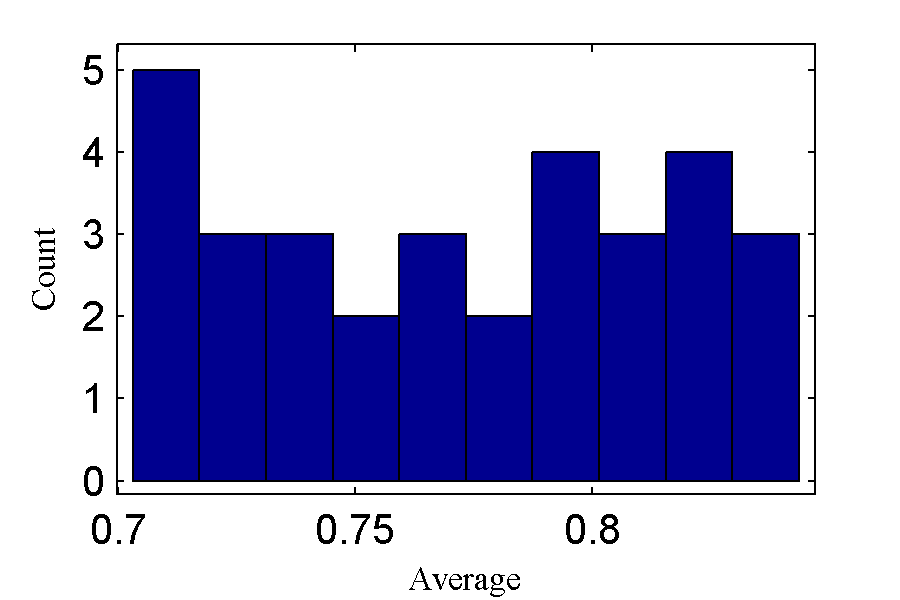
\includegraphics[width=\mywidth]{figs/hist_c1_block1_page1_withoutkey.png} 
%\includegraphics[width=3.0in]{figs/eval_performance_diff_context.pdf} 
% \caption{Group average without the stego-key}
% \label{fig:withoutkey_page} 

% \end{center} 
% \end{figure} 

% \begin{figure} 
% \begin{center} 
% 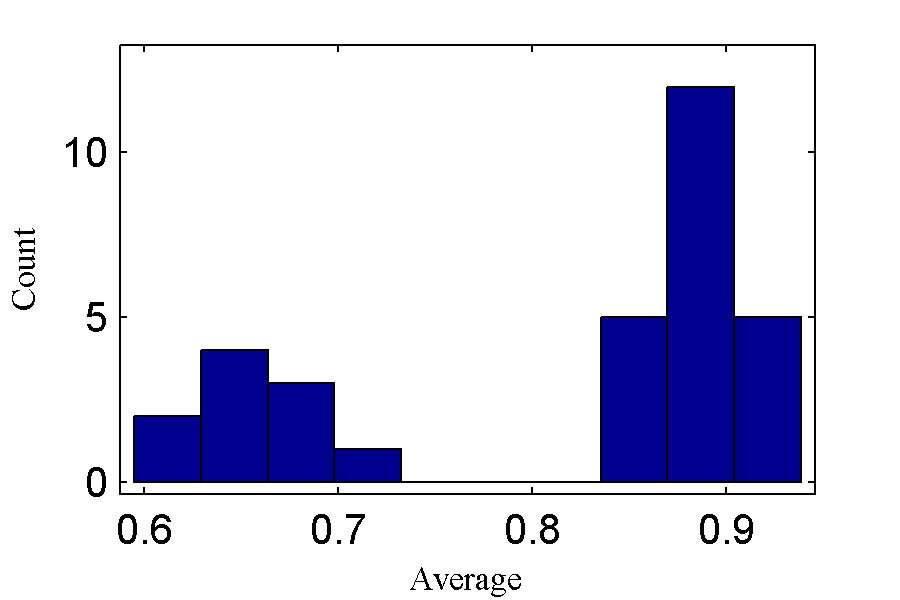
\includegraphics[width=\mywidth]{figs/hist_c1_block1_page1_withkey.png} 
%\includegraphics[width=3.0in]{figs/eval_performance_diff_context.pdf} 
% \caption{Group average with the stego-key}
% \label{fig:withkey_page} 

% \end{center} 
% \end{figure} 

%\begin{figure} 
%\begin{center} 
%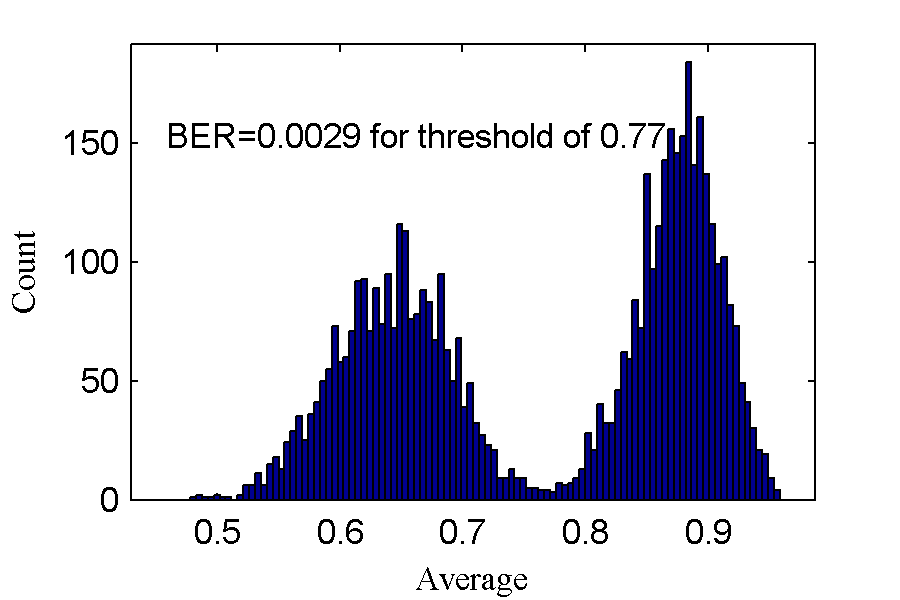
\includegraphics[width=\mywidth]{figs/5e3_histo_withkey.png} 
%%\includegraphics[width=3.0in]{figs/eval_performance_diff_context.pdf} 
%\caption{The distribution of the average program time of a group with 
%the stego-key.}
%\label{fig:withkey_10blocks} 
%\vspace{-0.1in}
%\end{center} 
%\end{figure} 

%To recover hidden information from the program time distribution,
%the intended recipient with the stego-key can compute the average
%program time for each group after the first thresholding. 
%Figure~\ref{fig:withoutkey_10blocks} shows the distribution of
%the resulting average program time.
%In this figure, 5120 groups which represent 5120 embedded bits
%are shown. 
%As shown in the figure, these is an obvious gap in the distribution
%between the fast and slow groups. Therefore, the value of hidden bits 
%can be easily recovered through a simple thresholding. 
%We get a bit error rate (BER) of 0.0029 (0.29\%) in this case.
%%even when a single
%%quantization threshold ($X$) is used across all pages.

%To recover hidden information from the program time distribution,
%the intended recipient with the stego-key can compute the average
%program time for each group after the first thresholding. 
%Figure~\ref{fig:withoutkey_10blocks} shows the distribution of
%the resulting average program time.
%In this figure, 5120 groups which represent 5120 embedded bits
%are shown. 
%As shown in the figure, these is an obvious gap in the distribution
%between the fast and slow groups. Therefore, the value of hidden bits
%can be easily recovered through a simple thresholding. 
%We get a bit error rate (BER) of 0.0029 (0.29\%) in this case.
%%even when a single
%%quantization threshold ($X$) is used across all pages.


%\begin{figure} 
%\begin{center} 
%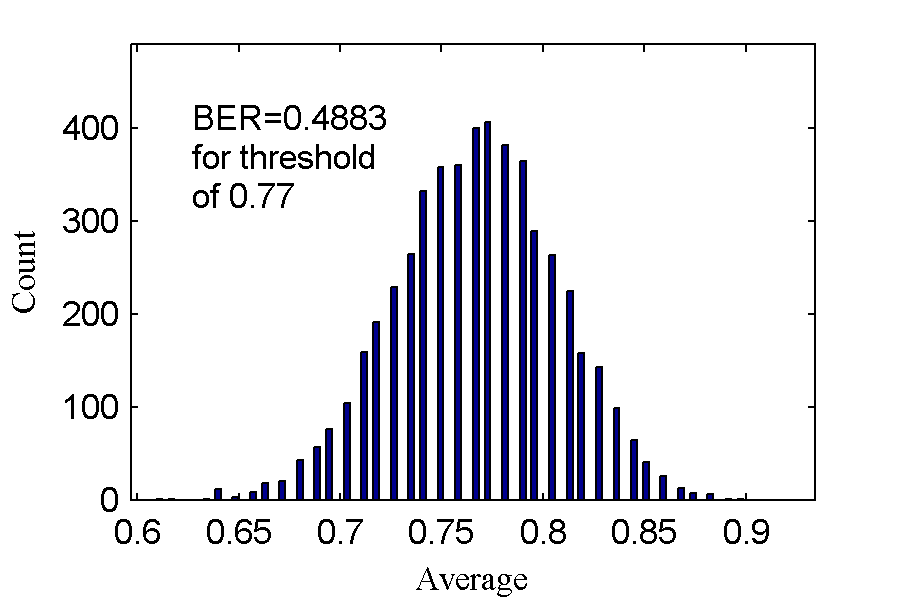
\includegraphics[width=\mywidth]{figs/5e3_histo_withoutkey.png} 
%%\includegraphics[width=3.0in]{figs/eval_performance_diff_context.pdf}
%\caption{The distribution of the average program time of a group
% without the stego-key.}
%\label{fig:withoutkey_10blocks} 
%\vspace{-0.1in}
%\end{center} 
%\end{figure} 

%On the other hand, Figure~\ref{fig:withoutkey_10blocks} shows the 
%distribution of the average program time when the stego-key is 
%unknown. In this experiment, we randomly selected groups. As shown 
%in the figure, the average program time of a group shows a normal 
%distribution without any clear separation between 1s and 0s. The BER 
%with the threshold $Th$ of 0.77 is 0.4883, which is close to 50\%. 
%This result suggests that an adversary cannot recover hidden 
%information without correct groupings because each group is likely 
%to have both more and less stressed bits.



%\begin{figure} 
%\begin{center} 
%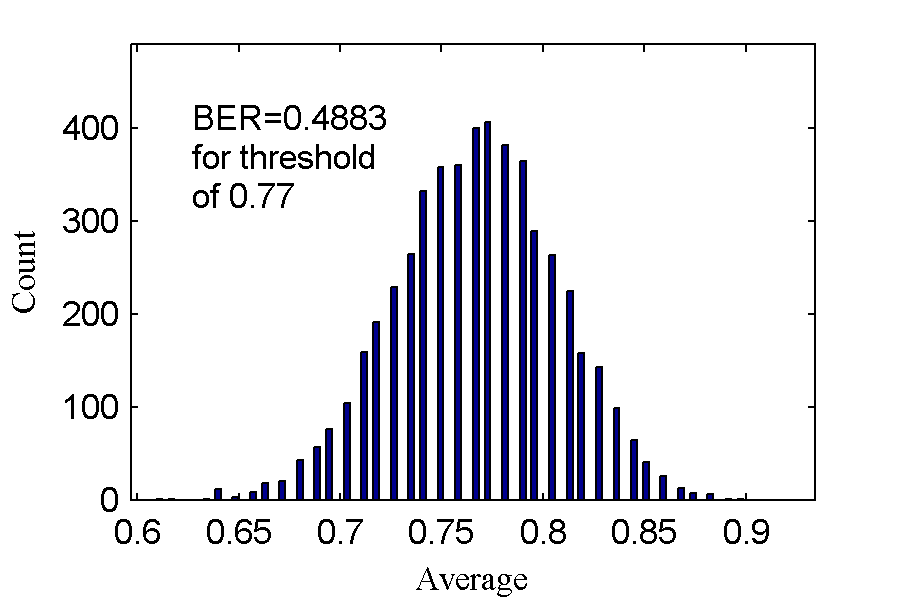
\includegraphics[width=\mywidth]{figs/5e3_histo_withoutkey.png} 
%%\includegraphics[width=3.0in]{figs/eval_performance_diff_context.pdf} 
%\caption{The distribution of the average program time of a group 
%without the stego-key.}
%\label{fig:withoutkey_10blocks} 
%\vspace{-0.1in}
%\end{center} 
%\end{figure} 

%On the other hand, Figure~\ref{fig:withoutkey_10blocks} shows the 
%distribution of the average program time when the stego-key is 
%unknown. In this experiment, we randomly selected groups. As shown
%in the figure, the average program time of a group shows a normal
%distribution without any clear separation between 1s and 0s. The BER
%with the threshold $Th$ of 0.77 is 0.4883, which is close to 50\%. 
%This result suggests that an adversary cannot recover hidden 
%information without correct groupings because each group is likely to
%have both more and less stressed bits.


\subsection{Robustness - Bit Error Rate}

In this subsection, we first study whether the proposed scheme can 
reliably hide and recover bits in the program time characteristics.
Here, we use the bit error rate (BER) as the metric for measuring 
robustness. To measure the BER, we hid a randomly generated message
into Flash memory and compared the retrieved message with the original.

In the baseline experiment, we used the first 4,096 bits of a page and
divided them into 32 groups (128 bits each) based on a randomly 
selected hiding key. Then, we selected multiple pages and blocks across
a Flash chip to form 5,120 groups, which represent 5,120 hidden bits,
and stored bits using 5,000 program and erase (PE) cycles in the encoding 
process. 
%Even though bits are intentionally stressed 5,000 times, as the figures
%show, there is no obvious bi-modal distribution between fast and slow
%bits. This results indicates that the inherent variation in program time
%across bits is much greater than the stress induced changes. The 
%distributions do not show a clear sign of hidden bits.
In this case, we got a bit error rate (BER) of 0.0029 (0.29\%).
%even when a single quantization threshold ($X$) is 
%used across all pages.

\begin{figure} 
\begin{center} 
\includegraphics[width=\mywidth]{figs/accuracy.png} 
\caption{Influence of hiding stress on BER.}
\label{fig:BER_vs_stress} 
\vspace{-0.1in}

\end{center} 
\end{figure}


Figure~\ref{fig:BER_vs_stress} shows the BER as a function of 
hiding stress, which is the number of program/erase (PE) cycles used
to stress each group in the hiding process. 
The blue line shows the average BER using a single Micron 4Gbit chip.
For each data point in the figure, the BER is computed over 5,120 
bits of hidden information with the group size of 128 bits.
For hiding stress levels of 2,500 and 5,000 PE cycles, we also show
the statistics across 15 Flash chips; the red triangles show the 
average BER and the error bars show the maximum and minimum BERs across 
the 15 chips. We can see that the BER decreases as the hiding stress 
increases. More stress increases the program time difference between
bits hiding 1s and 0s. However, the incremental benefit after 
5,000 PE cycles is rather small. Note that the typical lifetime
of an SLC Flash chip from the datasheet is 100,000 PE cycles. 

\begin{figure} 
\begin{center} 
\includegraphics[width=\mywidth]{figs/groupsize.png} 
\caption{Influence of group size on BER.}
\label{fig:groupsize} 
\vspace{-0.1in}

\end{center} 
\end{figure}


\begin{figure} 
\begin{center} 
\includegraphics[width=\mywidth]{figs/page_intv.png} 
\caption{Influence of page interval on BER.}
\label{fig:pageintv} 
\vspace{-0.1in}

\end{center} 
\end{figure}

There is also a trade-off between the robustness of the scheme 
and its hiding capacity. When more physical bits are included 
in a group, the capacity decreases. On the other hand, the 
statistical variations among groups will decrease as the group size
increases. Therefore, the BER decreases with an increasing 
group size, as shown in Figure~\ref{fig:groupsize}.  
It is also observed that neighboring pages have a strong influence 
on each other; stressing one page may also cause some stress in a 
neighboring page. To solve this problem, only a subset of pages with
a specific interval $K$ can be used within a block. If $K$ is 4, then only
page 0, page 4, page 8, and so on are used to hide information while
the rest is not used. The influence of this page interval on the BER 
is shown in Figure~\ref{fig:pageintv}. The experimental results suggest
that there is not much benefit to using a group size beyond 128 and a 
page interval beyond 4 for these chips. Figure~\ref{fig:groupsize}
and Figure~\ref{fig:pageintv} were generated from the 2Gbit Micron 
chips, but we found that the group size of 128 and page interval 
of 4 also work well for the 4 Gbit chips.

\begin{figure} 
\begin{center} 
\includegraphics[width=\mywidth]{figs/initialstess.png} 
\caption{Influence of initial stress level on BER.}
\label{fig:initial_stress} 
\vspace{-0.1in}

\end{center} 
\end{figure}

The effectiveness of the method on moderately used Flash chips is also
studied. The influence of the initial stress level before the encoding
process on the BER is shown in Figure~\ref{fig:initial_stress}. 
Here, we aim to simulate the normal usage of the Flash chip. 
So, in each program operation for the initial stress, random data are 
programmed. For example, the BER at the initial stress level of 10 PE 
cycles shows the error rate when bits are hidden after 10 PE cycles of
programming random data.
It can be observed that as the initial stress level increases, 
the BER also increases. 
However, a higher initial stress level can be tolerated by increasing
the stress level in the encoding process.
Note that the error rate is still manageable (less than 10-15\%) even 
after hundreds of normal PE cycles.

\begin{table}
  \begin{center}
    %\begin{scriptsize}
\begin{tabular}{|l|c|c|}
\hline

  & 5,000 Hiding PE & 10,000 Hiding PE \\

\hline
BER after zero retention  & 0.0029 & 0.0021 \\
(1 post PE cycle) & &\\
\hline
BER after 2-day retention &  0.0141 & 0.0035 \\
(3 post PE cycles) & &\\
\hline
BER after 3-day retention & 0.0187 & 0.0045 \\
(5 post PE cycles) & &\\
\hline
BER after over a month & 0.0178 & 0.0031 \\
retention(7 post PE cycles) & &\\
 \hline

\end{tabular}
%\end{scriptsize}


  \end{center}
\vspace{-0.1in}
\caption{Retention characteristics of the hidden message.}
\label{tab:retention}
\vspace{-0.2in}
\end{table}


The retention characteristics of the hiding scheme are shown 
in Table~\ref{tab:retention}. Note that since each decoding 
performs 2 PE cycles, these retention characteristics include
impacts from additional PE cycles in addition to the time
between information hiding and retrieval.
In the first three rows of Table~\ref{tab:retention}, the BER
increases as retention time and post-hiding PE cycles increase. 
In the last row, the BER actually decreases a little compared to the 
third row. 
%Considering that the additional PE cycles reduce the
%intentional biases and increase the BER, we can conclude that the
%retention time has little effect on the BER. 
The results suggest that the retention time has little effect on
the BER.
Intuitively, given that the hiding scheme utilizes cell aging, 
this result is also supported by the fact that a worn-out Flash
memory does not recover greatly even after having been left
unattended for a long time. 


\subsection{Performance}
\label{sec:perf}


In our experiments, when a whole page is used for hiding, 
it takes about 123.6 seconds to perform 5,000
PE cycles of hiding stress on a block, which embeds 2,048 bits of
information in the block. The hiding throughput is around 16.6
bits/second. The upper limit of the throughput can also be calculated using the page
program time and block erase time given in the Flash memory chip
datasheet. The typical page program time is 200 microseconds and
the typical block erase time is 700 microseconds. With 2,048 hidden bits
in 16 pages of a block, the 5,000 PE cycles will take 
$(0.2*16+0.7)*5,000/1,000=19.5$ seconds. The throughput will be about 
105 bits/second. This is the ideal case which does not include 
program data transfers and microcontroller overhead. 
The hiding throughput will also be higher if we use a smaller number of
PE cycles for stressing, or if we use smaller groups. 

%\textbf{TODO: is this presentation reasonable?.}
In order to read the hidden information, one needs to obtain per-bit 
program times using partial programming. The characterization speed depends 
on the number of partial programs, $M$, used in the decoding algorithm. 
For reading hidden bits (decoding), we only need to perform partial programs 
until more than half of the bits flip. 
In our experiment, $M$ for decoding is around 30, 
and it takes around 3.63 seconds to characterize 16 pages, which contain 
2,048 hidden bits. Therefore, the read throughput is about 564 bits/second.  
The read throughput will be higher if the hiding scheme uses a smaller number of
Flash bits to encode each hidden bit.
%When a group has smaller number of cells, the read throughput will be
%higher as we can get more decoded bits out of the same 
%number of Flash bits.
%Still, $M$ depends on the time used for each partial 
%program, $T$. 

For a detailed analysis to detect hidden bits (see \ref{ssec:perbit-analysis}),
one needs to obtain a complete program time distribution with a large $M$. 
In our testbed, it takes 612.6 seconds to characterize a block using 
$M = 1,200$ even if we ignore data transfer from the microcontroller to the host
computer and processing time on the host.
%On average, it takes 2.3 seconds to characterize 4,096 bits in a page.
%If each group has 128 cells, then the 4,096 Flash bits provide 32 bits 
%of hidden information.
%Therefore, the read throughput is about 13.88 bits/second. 
%The typical random read latency is 25 microseconds which is
%quite small compared to 2.3 seconds.
%\textbf{This section needs better numbers.}
%If we use the entire page, which has four times more bits than 
%4,096 bits, obtaining the per-bit program time will take around 
%9.2 seconds. Read throughput will also increase by four times, 
%in this case with a 128 bit group size, to 55.5 bits/second. 
%\textbf{TODO: IS THIS TRUE?} 
A 4Gbit Flash memory chip has 
4,096 blocks, so obtaining the complete program time distribution
of the whole chip will take around 29 days. 
%For decoding,
%it takes around 16.5 hours. 
Higher capacity chips will take even more time to characterize for detection
and decoding. For comparison, simply reading
the digital content from the 4Gbit Flash chip will take approximately 4 minutes. 
Therefore, fully characterizing the entire Flash chip without knowing
where hidden information is located is quite time consuming.

%Suppose one page out of four pages are selected for hiding and each
%group has 128 cells. Then we can hide 1/512 of the
%flash memory chip capacity of raw data. The capacity should be 
%optimized with comprehensive analysis on selected page interval,
%group size and BER which require extra ECC bits.


\subsection{Detectability}

The previous subsection shows that the per-bit program time in Flash memory
can be controlled sufficiently to reliably store hidden 
information. Here, we 
discuss whether an attacker with access to a Flash chip can detect the 
existence of hidden information. In essence, the question is 
whether variations in Flash memory characteristics due to information 
hiding can be distinguished from variations due to normal use. 

The proposed information hiding scheme uses per-bit program time,
which is not visible from the digital content 
in a Flash memory device. Also, the hiding 
operation does not change normal Flash
functions; users can still read, erase, and write Flash memory
in the expected manner.
Therefore, the hidden information cannot be detected from the 
inspection of digital content. Instead, an attacker 
needs to rely on checking the analog properties of the Flash memory.

The following list summarizes the steps that an attacker needs to 
take in order to analyze the analog properties, and in particular, 
the timing properties, of Flash memory.

\begin{enumerate}
\item Check for anomalies in timing of normal Flash operations. 

\item Pick pages/blocks for more detailed analysis.

\item Collect per-bit program time for a selected page.

\item Analyze the per-bit program time distribution of a page.

\item Repeat Steps 2 to 4.

\end{enumerate}

In order to determine whether a Flash chip contains hidden information or not,
an attacker can start by checking the timing of normal Flash operations such as
per-page program time and per-block erase time, which can easily be obtained 
from normal operation. If these operations do 
not show any anomaly -- their timing is within the range of timing 
characteristics for normal use -- then the
attacker needs to obtain and analyze per-bit program time by picking a page for
detailed analysis, collecting per-bit program times through partial programs,
and
then running an analysis. If there is no way to identify suspicious pages and blocks
from normal operations, in the worst case,
the attacker will need to perform the detailed analysis for every single page in Flash 
memory, which will take a long time.
%in a brute-force fashion.

%by brute forcing selection of group size and hiding key in order 
%to determine if a page has hidden data is, and then what that data would be.
%The analog characterization process itself for an entire chip 
%takes a long time (estimated 29 days for the chips used). The cryptoanalysis,
%using group size and hiding key, scales exponentially. If the attacker does
%not know which chip has hidden information on it, characterizing every
%Flash chip that they can reach would be a very slow process.
%Also, an absence of
%this length would be noticed by the hiding party and mitigating steps could be
%taken.
%\textbf{TODO: sort of a weak plan for the hiding party... if that information
%iscritical?}

In the rest of the subsection, we will discuss each step that the attacker
needs
to take and whether the information that is hidden can be 
detected in each step.


\subsubsection{Anomalies in Normal Flash Operations}

%\begin{figure} 
%\begin{center} 
%\includegraphics[width=\mywidth]{figs/c6_readtime_aftererase.png} 
%\caption{Read time histogram after block erase. The histogram after page program is similar.}
%\label{fig:rtime_afterprogram} 
%\end{center} 
%\end{figure}

%\begin{figure} 
%\begin{center} 
%\includegraphics[width=\mywidth]{figs/c6_readtime_afterprogram.png} 
%\caption{Read time histogram after page program.}
%\label{fig:rtime_aftererase} 
%\vspace{-0.1in}
%\end{center} 
%\end{figure}


%\begin{figure} 
%\begin{center} 
%\includegraphics[width=\mywidth]{figs/ptime_normalusage.png} 
%\caption{Program time for pages within a block, normal usage.}
%\label{fig:ptime_normal} 
%\end{center} 
%\end{figure}

%\begin{figure} 
%\begin{center} 
%\includegraphics[width=\mywidth]{figs/ptime_hiding.png} 
%\caption{Program time for pages within a block, with hiding.}
%\label{fig:ptime_hide} 
%\vspace{-0.1in}
%\end{center} 
%\end{figure}

%\begin{figure} 
%\begin{center} 
%\includegraphics[width=\mywidth]{figs/avgptime_regular.png} 
%\caption{Average page program time for normal usage.}
%\label{fig:avgptime_normal} 
%\vspace{-0.1in}
%\end{center} 
%\end{figure}

%\begin{figure} 
%\begin{center} 
%\includegraphics[width=\mywidth]{figs/avgptime_hide.png} 
%\caption{Average page program time for hiding.}
%\label{fig:avgptime_hide} 
%\vspace{-0.1in}
%\end{center} 
%\end{figure}

%\textbf{TODO: need to standardize on "hiding
%PE cycles"; "normal PE cycles". Also "hiding pages".}


Stressing a Flash chip may affect the analog characteristics
of normal memory operations such as page read time, page program time, 
and block erase time. 
If these characteristics change significantly due to our scheme,
an attacker could use that to detect the existence of hidden 
information. Therefore, we first study the impact of information 
hiding and normal Flash use on the page read time, page program time, 
and the block erase time.

Using the Micron 4Gbit chips, we tested six hiding PE cycle counts 
(625, 1,250, 2,500, 5,000, 7,500, and 10,000) and five normal PE 
cycle counts (0, 32, 64, 128, 256) on 4 different chips. On each chip,
we used 20 blocks, 
each containing 64 pages. Because we hide data once every fourth pages, 
only 16 pages within each block are used to hide information.
A normal PE cycle is performed by writing randomly generated data 
to every page in a block, then erasing that block, simulating
wear from normal usage.

To study the impact of information hiding on the page read time,
we measured the time to read pages (after performing
an erase) when they were fresh as well as after 5,000 hiding PE cycles. 
%Figure~\ref{fig:rtime_aftererase}. Read times after a performing a program
%show a similar histogram.
%, and Figure~\ref{fig:rtime_afterprogram}. 
The read times were virtually identical before and after the hiding
stress, showing that the read time would not be a good indicator for 
the existence of hidden information.
%No obvious change caused by stress was visible here, with
%the distributions of fresh page read times and
%pages with hidden information read times coinciding well. 
%This result is expected and coincides with previous literature.

%To the eye it would be nearly impossible to differentiate 
%any existing deviation. 
%\textbf{TODO: I also put data from c3 into the figure directory. Do we want to use that?:}
%A more thorough analysis by support
%vector machine is considered later in the section.
%\textbf{TODO: IF THERE IS A CHANGE:} It appears that pages with hidden 
%information
%tend to have a significant increase in read time. A chip with
%many pages having a high read time could then be considered
%suspicious by an attacker and set aside for further study. 
%It is notable that since chip to chip variation is significant,
%a chip with many high read time pages could also be the
%result of process variation and/or normal usage, and -
%an attacker could only be certain after further analysis.

%figure for page program time within a block 2
%\begin{figure} 
%\begin{center} 
%\includegraphics[width=\mywidth]{figs/programtime_5000pe32pe.png} 
%\caption{Program time for 64 pages within a block (not sure whether want to show this one or previous one.}
%\label{fig:ptime_block2} 
%\vspace{-0.1in}
%\end{center} 
%\end{figure}

Figure~\ref{fig:ptime_block1} shows the program times for individual pages in two 
blocks from one chip, one fresh block and the other with hidden information. 
As shown in the figure, 
even though our hiding algorithm only uses every fourth page in a block,
there is no visible pattern in per-page program time.
The figure also shows that
the program time of a page shows distinct values. The distribution between
the distinct program times may change as a page wears out with PE cycles. However, 
we found that the possible program time values for each chip stay the same across 
the range of stress levels in both normal usage and information hiding cases.
%Therefore, each page's program time by itself does not show whether the page has
%hidden information or not. 

%figure for page program time within a block 1
\begin{figure} 
\begin{center} 
\includegraphics[width=\mywidth]{figs/programtime_block.png} 
\caption{Program time for pages within a block.}
\label{fig:ptime_block1} 
\vspace{-0.1in}

\end{center} 
\end{figure}

%program time histogram
\begin{figure} 
\begin{center} 
\includegraphics[width=\mywidth]{figs/programtime_hist.png} 
\caption{Program time histogram for three stress levels.}
\label{fig:ptime_histo} 
\vspace{-0.1in}
\end{center} 
\end{figure}


%figure for how the program time change with stress, hide
%\begin{figure} 
%\begin{center} 
%\includegraphics[width=\mywidth]{figs/programtime_hiding.png} 
%\caption{Program time for blocks with hiding.}
%\label{fig:ptime_hide} 
%\vspace{-0.1in}

%\end{center} 
%\end{figure}

%figure for how the program time change with stress, random
%\begin{figure} 
%\begin{center} 
%\includegraphics[width=\mywidth]{figs/programtime_normal.png} 
%\caption{Program time for normal blocks.}
%\label{fig:ptime_random} 
%\vspace{-0.1in}

%\end{center} 
%\end{figure}



%\textbf{OLDER DATASET not shown: For the Micron 4G bit chips, 
%we tested 6 chips. For each chip, we tested
%10 blocks for each hide stress level (625, 1250, 2500, 5000, 7500
%and 10,000 PE cycles), 100 fresh blocks, and 5 blocks for each random stress
%level from 1 random PE cycle to 4096 random PE cycles.}
%The histograms for program time and erase
%time are shown in Figure~\ref{fig:ptime_4gchip} and
%Figure~\ref{fig:etime_4gchip}.
Figure~\ref{fig:ptime_histo} shows the program time distributions across
four chips for three different stress levels: fresh, 5,000 hiding PE cycles,
and 32 normal PE cycles. The figure again shows that the program time falls
into a small set of distinct values even though there are more distinct values 
across 4 chips. More importantly, pages with and without hidden information share 
the same set of program time values. 
Also, unlike per-bit program time, the experimental results show that 
the page program time does not change significantly with stress, at least
for the particular 4Gbit chips that we tested.
This is likely due to the fact that the page program time is determined by the
control circuit based on the slowest bit within a page.
Therefore, each page's program time by itself does not show whether the page has
hidden information or not. 

%Therefore, each page's program time by itself does not show whether the page has
%hidden information or not. 

%We can see that for the 4G chips, the page program time is almost 
%not influenced by stress to the eye. We also examine this metric
%later in an SVM. 

%figure for how the erase time change with stress, hide
%\begin{figure} 
%\begin{center} 
%\includegraphics[width=\mywidth]{figs/erasetime_hiding.png} 
%\caption{Erase time for blocks with hiding.}
%\label{fig:etime_hide} 
%\vspace{-0.1in}
%\end{center} 
%\end{figure}

%figure for how the erase time change with stress, random
%\begin{figure} 
%\begin{center} 
%\includegraphics[width=\mywidth]{figs/erasetime_normal.png} 
%\caption{Erase time for normal blocks.}
%\label{fig:etime_random} 
%\vspace{-0.1in}

%\end{center} 
%\end{figure}


%\textbf{TODO 4Gbit erase time data/discussion.}
Figure~\ref{fig:etime_chip1} and Figure~\ref{fig:etime_histo} illustrate the block
erase time distribution within a chip and across 4 chips, respectively.
Similar to the program time, the erase time also falls into a few distinct levels,
which are common across different stress levels. On the other hand,
the figures show that the erase time tends to increase as the stress level
increases. As a result, blocks with hiding stress are more likely to have
a long erase time compared to fresh block without any stress. In that sense,
the erase time may be used to distinguish fresh pages from blocks with hidden bits. 
However, because both normal PE cycles and hiding PE cycles increase
the erase time, it is unclear how to distinguish blocks with hidden information
from blocks with normal PE stress based on the erase time distribution
(see Figure~\ref{fig:etime_histo}). 
We also found that there exist fairly large chip-to-chip variations.
For example, some fresh chips may have over 50\% of blocks that show a long
erase time even without any PE stress. 

%figure for erase time within a chip 1
\begin{figure} 
\begin{center} 
\includegraphics[width=\mywidth]{figs/erasetime_block.png} 
\caption{Erase time for 20 blocks within a chip.}
\label{fig:etime_chip1} 
\vspace{-0.1in}

\end{center} 
\end{figure}

%erase time histogram
\begin{figure} 
\begin{center} 
\includegraphics[width=\mywidth]{figs/erasetime_hist.png} 
\caption{Erase time histogram for three stress levels (across 4 chips).}
\label{fig:etime_histo} 
\vspace{-0.1in}

\end{center} 
\end{figure}

%for fresh chips, some chips have few blocks that show larger erase time while
%others have
%a lot of blocks (over 50\%) show bigger erase time. So it is hard to tell
%whether a chip
%with a lot of blocks with bigger erase time has hidden information or not.
%%Further more,
%%even within the same chip, the increase in number of blocks with bigger erase
%%time is
%%negligible under stress level 7500 PE cycles for most of the chips. 
%Since both
%normal blocks
%and blocks with hidden information can have a smaller or bigger block erase
%time, the block
%erase time can not be used for detection based on simple inspection.
 
%The changes of block 
%erase time with hiding and normal stress are shown in Figure~\ref{fig:etime_hiding} 
%and Figure~\ref{fig:etime_normal}, respectively.

%\begin{figure} 
%\begin{center} 
%\includegraphics[width=\mywidth]{figs/erase_time_normal.png} 
%\caption{Erase time for normal blocks, 2Gbit chips.}
%\label{fig:etime_normal} 
%\vspace{-0.1in}

%\end{center} 
%\end{figure}

%\begin{figure} 
%\begin{center} 
%\includegraphics[width=\mywidth]{figs/erase_time_hiding_part.png} 
%\caption{Erase time for blocks with hiding, 2Gbit chips.}
%\label{fig:etime_hiding} 
%\vspace{-0.1in}

%\end{center} 
%\end{figure}

%\textbf{TODO: SVM analysis of page read time, program time, and erase time
%for 4Gbit chips}

The experimental results so far show that there is no obvious pattern in program time 
and erase time distributions to distinguish pages or blocks with hidden information
from pages or block with normal PE stress. 
Yet, it may be possible that there exists a pattern that is difficult to detect
in human eyes. To further study detectability of hidden information based on
normal Flash operations timings, we tried a support vector machine
(SVM) to predict whether a page or a block has hidden information.
A support vector
machine is a machine learning model that is widely used to recognize patterns and
classify data sets. We used libsvm, a popular SVM software package
\cite{libsvm}. 

%The goal of the SVM is to classify a page/block correctly, without
%knowing a priori if a page/block has hidden data or not. 
For the SVM experiments, we constructed multiple data sets using pages/blocks
with hidden information as well as pages/blocks with normal stress, combining
data from one hiding stress level and one normal stress level. We used
two hiding stress levels (2,500 and 5,000 PE cycles) and five normal stress
levels (0, 32, 64, 128, 256 PE cycles), collected from 4 Flash chips.
Then, for each data set, the SVM was trained with data from
3 chips and then tested on data from one remaining chip. 
This construction represents an idealistic scenario for an attacker.
In practice, the attacker will need to consider all possible stress levels for 
both normal uses as well as hiding, which will add more variations.


\begin{figure} 
\begin{center} 
\includegraphics[width=\mywidth]{figs/per_page_svm.png} 
\caption{SVM accuracy for detecting hidden information (per-page analysis).}
\label{fig:page_svm} 
\vspace{-0.1in}

\end{center} 
\end{figure}


\begin{figure} 
\begin{center} 
\includegraphics[width=\mywidth]{figs/per_block_svm.png} 
\caption{SVM accuracy for detecting hidden information (per-block analysis).}
\label{fig:block_svm} 
\vspace{-0.1in}

\end{center} 
\end{figure}


Figure~\ref{fig:page_svm} shows the prediction accuracy when the SVM is given
the program time and erase time for each page individually without a notion of
blocks.
The SVM performs relatively well when distinguishing fresh pages and pages
with hiding stress.
However, the accuracy drops significantly when comparing pages with hiding stress
and pages with moderate levels of normal PE stress. In such cases, the accuracy
is not much better than random guesses (50\%).
The SVM performs better again for cases with high normal stress levels beyond 
128 PE cycles because the normal stress exceeds the hiding stress level.
In essence, the results suggest that the SVM can distinguish pages with different
stress levels, but not pages with hiding stress and normal stress.

Figure~\ref{fig:block_svm} shows the accuracy of another SVM construction
where the input vectors were organized by block. In this design, each input 
is a vector of program and erase time pairs for each page within a block, 
allowing the SVM to see a pattern within a block instead of handling each
page separately. The goal of this SVM is to identify blocks with hidden
information. The accuracy of this SVM was similar to that of the 
per-page SVM. The SVM could distinguish more stressed blocks from less stressed
blocks, but not the hiding stress from the normal stress.

While not shown here, we also tested cases where data from all stress levels
were combined together to form a large data set. We found that dealing with
multiple stress levels significantly reduces SVM prediction accuracy for
both the page-granularity analysis and the block-granularity analysis.
The SVM predictions were no better than random guesses.


%\textbf{TODO: the following text corresponds to point 3 in my summary, which notes
%that chip to chip, block to block, page to page, and model to model variation
%is significant too!}


%Although a quick examination of the erase time (with stress level knowledge)
%could indicate a block/chip with hidden data, it is important to note
%that all detected values still fall within the values expected
%from a normally used chip. These values can be highly variable even within
%a chip itself. Blocks and pages in the same chip can show incredible variability
%in program and erase times and in the manner they respond to 
%program and erase stress \textbf{TODO should we cite characterization work?}. 

The experimental results so far show that it is difficult to distinguish pages/blocks
with hiding stress from pages/blocks with normal stress even on one particular
Flash model (Micron 4Gbit). In practice, an adversary will also need to deal with
diversity and variations among multiple Flash manufacturers and models, which will make
detecting hidden bits even more difficult.

In fact, we found that analog characteristics of Flash memory varies significantly
from model to model.
%Although the results suggest that it is more likely that a block with hidden data on it
%would have a higher erase time, this result is only valid for this particular model
%of Flash memory chip. Model to model variation is an important concern for this
%type of analysis. Because there is significant variation
%between models, the behavior of different models can vary greatly and assumptions
%from one model do not necessarily carry over to another.
For example, we tested 2Gbit Flash chips from Micron, which have an identical
specification with the 4Gbit chips except for the capacity. 
%Compared to the Micron 4Gbit chips, their 
%datasheets indicate identical specs but for one difference: the 2Gbit chips have feature 
%set E (fifth generation) while the 4Gbit chips have feature set D 
%(fourth generation), as shown in the product part number. 
Surprisingly, the 2GBit chips, although only a generation apart from
the 4Gbit chips, showed a markedly different behavior compared to the 4Gbit chips. 
For 2Gbit chips, the PE stress had little impact on block erase time
while noticeably changing page program time. In essence, the 2Gbit chips showed
the opposite type of behavior as the 4Gbit chips where the erase time shows
a significant shift. In both cases, we still found that it is difficult to distinguish
the impact of hiding stress from that of normal stress. 

%Almost no difference was seen in the erase times of blocks
%with hidden data and blocks stressed normally, but 
%significant variation did exist in the distributions of program times 
%of hidden vs. normally used pages. In essence, the 2Gbit chips showed
%the opposite type of behavior as the 4Gbit chips.

The significant variations across Flash models imply that an attacker will
need to build and train an SVM model for each Flash chip model in order to use the SVM
for determining the existence of hidden data on a particular chip. 
%The significance of this finding is that for an attacker to
%use normal Flash operation times to 
%determine the existence of hidden data on a particular chip,
%an SVM model would 
%have to be built and characterized for every type of Flash
%chip in which they are interested. 
Obviously, this would require a significant investment on the part of the attacker.
Even then, as we have shown above, there is no guarantee that an SVM
model using normal Flash operations 
will be able to determine the existence of hidden data with a high
probability.

%One thing to note is that for different generations of chips, even two products 
%from the same manufacturer and with very similar specifications, the normal page 
%program time and block erase time can show very different behaviors 
%with stress. 

% MICRON 2Gbit test conditions -- leave them out here?
%For the Micron 2Gbit chips, we tested 5 blocks, each having 64 pages,
%for each hiding stress level and normal PE cycles (writing random data).
%We used 625, 1250, 2500, 5000 and 10000 hiding PE cycles, and 1, 10, 100, 
%and 1000 normal usage.

%\textbf{TODO this page program time section is from the 2Gbit chip data
%and lifted from what we had before.}
%Second, for page program times, we found that a program time of a page
%always shows one of two distinct values for all stress levels in
%normal usage and hiding processes.
%As the stress level (the number of PE cycles) 
%increases in both normal usage and hiding, the number of pages
%with a longer program time decreases and the number of pages with
%a shorter program time increases. Figure~\ref{fig:ptime_normal}
%shows the page program times for pages in two blocks with normal
%stress and Figure~\ref{fig:ptime_hide} shows the page program
%time for pages in another two blocks with hidden information. From the two
%figures, we can see that the two distinct values for page program time
%are the same across the stress levels in both normal
%usage and information hiding. We can also see that even though a
%fixed page interval is used to hide information within a block,
%this does not create a regular pattern of page program times for
%pages within a manipulated block.

%To measure the increase in the number of pages with a shorter page
%program time when the stress level is increased, the average page
%program time is plotted. Figure~\ref{fig:avgptime_normal} shows
%the average page program time in the normal usage situation and
%Figure~\ref{fig:avgptime_hide} shows the average page program
%time with hidden information. The two figures show that the
%stress level has a bigger influence on the page program time in
%the regular usage situation than in the hiding situation.
%Therefore, even though the blocks with hidden information
%experience more PE cycles, they are indistinguishable from
%moderately used blocks under normal usage from the perspective of 
%page program time.

%At the circuit level, this result is expected because the
%page program time is determined by the few slowest programming
%bits in a page. In normal usage, almost every bit is
%programmed to 0 in about a half of PE cycles. In the hiding process, nearly
%half of the bits are only programmed to 1. Therefore, the
%programming speed of the slowest programming bits in regular
%usage should increase faster than the slowest programming bits
%used to hide information. Note that the range of the average program
%times for the pages used to hide information (1.70 to 1.86 s) is completely
%contained in the range of program times for pages used normally (1.66 to 1.88
%s).



%\textbf{TODO: this discussion is for 2Gbit chips.}
%The block erase time for blocks under normal usage and blocks
%used for hiding information are shown in
%Figure~\ref{fig:etime_normal} and Figure~\ref{fig:etime_hiding},
%respectively. 
%We can see
%that for hiding stresses up to 10,000 PE cycles, the block erase
%time for manipulated blocks is indistinguishable from blocks
%under normal usage. 
%This result suggests that the hiding scheme with 10,000 PE cycles
%or less cannot be detected by looking at the erase time distribution.

%%But for a hiding stress of 20,000 PE cycles and
%%40,000 PE cycles, there is a noticeable increase in block erase time.
%%For 20,000 PE cycles, some manipulated blocks are
%%indistinguishable, as seen from the minimum value of the block
%%erase times. For 40,000 PE cycles, most of the manipulated blocks
%%have a higher block erase time than moderately used blocks.
%%Yet, a high PE stress beyond 10,000 cycles should 
%%only be used when the adversary is not explicitly checking the 
%%erase time.

%\begin{figure} 
%\begin{center} 
%\includegraphics[width=\mywidth]{figs/programtime_histo.png} 
%\caption{Program time distribution for Micron 4G chip.}
%\label{fig:ptime_4gchip} 
%\vspace{-0.1in}

%\end{center} 
%\end{figure}

%\begin{figure} 
%\begin{center} 
%\includegraphics[width=\mywidth]{figs/erasetime_histo.png} 
%\caption{Erase time distribution for Micron 4G chip.}
%\label{fig:etime_4gchip} 
%\vspace{-0.1in}

%\end{center} 
%\end{figure}

\subsubsection{Page Selection and Per-Bit Program Time Collection}

%\textbf{TODO: NOTE: This section largely unchanged.}


%Determining which pages have hidden data on them by inspection of their read,
%program, and erase times is difficult because hidden pages have values that 
%fit within
%the noise of normally used pages. Our experiments showed that a hiding PE of
%5,000 cycles was low enough to remain hidden in the noise of the normally used
%pages, allowing them to remain indistinguishable from fresh pages or moderately
%used pages.

%If a higher hiding PE cycle count is used, then it may become obvious which pages have been
%used to hide data. In this case, other pages (up to the entire chip) could be
%stressed to a similar level, thereby cloaking the hidden page again. This would
%slow down the hiding process, however.

% WE NEED TO GIVE MORE DETAILED RESULTS, NOT JUST A CLAIM.
%As we have seen, there is no certainty that blocks with hidden information 
%can be determined from 
The study of normal Flash operations shows that an adversary cannot simply determine
whether a Flash chip has hidden information or not based on measurements of normal 
Flash operation times. In essence, the hiding stress cannot be effectively distinguished 
from normal PE stress. As a result, an attacker needs to perform a more detailed
analysis on per-bit program times in an attempt 
to determine the existence of hidden data, which we will discuss next.

%Without a fast and effective way to identify potential pages or blocks with 
%hidden information, an adversary
To perform the detailed analysis of each page, the attacker will have to
characterize each page. However, characterizing per-bit program time for every page is 
quite a time-consuming process. As discussed in 
Section~\ref{sec:perf}, a 4 Gbit Flash memory chip requires around 29 
days to characterize. For larger chips, which are common today, the per-bit characterization
will take even longer. 

%While an analysis of normal Flash operation times may not provide enough certainty
%in the detection of hidden information, it may be able to provide candidate locations 
%for an attacker to examine more closely. 
To avoid expensive characterization of every page, an attacker may be able to use
normal Flash operation times to select candidate pages for the detailed analysis.
For example, for the 4Gbit Micron chips, an attacker 
may consider blocks with a higher erase time to be more likely to have hidden information.
%An attacker could start by selectively characterizing these blocks at
%the per-bit program time level. We note that it is possible 
%that blocks with hiding stress can be disguised 
%by stressing other blocks on the chip with a moderate number of normal PE 
%cycles.
However, the study in the previous subsection suggests that pages and blocks with hiding
stress can be hidden by stressing other blocks on the chip with a moderate number of normal PE 
cycles. 
%Some blocks with hidden information will not show up with a 
%higher erase time and could be missed. 

%The only way to be 
%certain would be to collect per-bit program times for every page.

%Note that after per-bit program time collection, there remains the need to crack the
%hiding key to discover the existence of any hidden information.

\subsubsection{Per-Bit Program Time Analysis}
\label{ssec:perbit-analysis}

%\begin{figure} 
%\begin{center} 
%\includegraphics[width=\mywidth]{figs/10rpe_histo_normalusage.png} 
%\includegraphics[width=3.0in]{figs/eval_performance_diff_context.pdf} 
%\caption{Partial program time distribution for bits in a page
% with 10 normal PE cycles only.}
%\label{fig:hist_10penormal} 
%\vspace{-0.1in}

%\end{center} 
%\end{figure}

%\begin{figure} 
%\begin{center} 
%\includegraphics[width=\mywidth]{figs/100rpe_histo_normalusage.png} 
%\includegraphics[width=3.0in]{figs/eval_performance_diff_context.pdf} 
%\caption{Partial program time distribution for 
%bits in a page with 100 normal PE cycles only.}
%\label{fig:hist_100penormal} 
%\vspace{-0.1in}

%\end{center} 
%\end{figure}

\begin{figure} 
\begin{center} 
\includegraphics[width=\mywidth]{figs/histo_compare.png} 
%\includegraphics[width=3.0in]{figs/histo_compare.png} 
\caption{Partial program number distribution curve averaged over 5 blocks.}
\label{fig:histo_comp} 
\vspace{-0.1in}

\end{center} 
\end{figure}

A more detailed detectability analysis involves analyzing the partial program
time distribution for bits within a page. In normal usage, the bits are
programmed 0s and 1s randomly over time. In the hiding scheme, some bits are
always programmed 0s and others are always programmed 1s. However, the hiding
scheme does not cause an obvious bimodal distribution due to large intrinsic
variations of bits in a page. Figure~\ref{fig:histo_comp} shows the partial
program time distribution averaged over 5 blocks. It can be seen that they are
very similar to each other.

To statistically analyze the distributions, we turned to support vector
machines again. To train an SVM for the per-bit analysis,
we prepared pages across 2 different hiding PE stress levels (2,500 and 5,000)
and 8 different normal wear stress levels (32, 64, 128, 256, 512, 1,024, 2,048, and 
4,096 PE cycles). We used 5 blocks on each chip, 16 pages per block, for a total
of 80 pages per chip, at each stress level; i.e. on one
chip, there are 80 pages with a hidden message stressed at 2,500 hiding PE
cycles, 80 pages with a hidden message stressed at 5,000 hiding PE cycles, 80
pages without hidden data stressed 32 normal PE cycles, and so on. We
characterized pages across 15 different chips. Each page represents a data
point in the SVM. The SVM had access to the complete raw data for each page: the
vector representing a page and an entry for each bit, with the entry's value as
the partial program time.

We then grouped the data from all chips into multiple sets, combining one hiding 
stress level and one normal stress level.
For example, one data set comprises the hidden data with 2,500 hiding PE
cycles and the data with 128 normal PE cycles, another data set used 5,000 PE
hidden data and 4,096 normal PE cycles, and so on, with a data set for each
combination of hiding and normal PE cycles.

\begin{figure} 
\begin{center} 
\includegraphics[width=\mywidth]{figs/svm_rawdata.png} 
\caption{SVM accuracy for detecting pages with hidden information (using raw data).}
\label{fig:svm_acc1} 
\vspace{-0.1in}
\end{center} 
\end{figure}

\begin{figure} 
\begin{center} 
\includegraphics[width=\mywidth]{figs/svm_stat_moments.png} 
\caption{SVM accuracy for detecting pages with hidden information (using statistical moments).}
\label{fig:svm_acc2} 
\vspace{-0.1in}
\end{center} 
\end{figure}

For each data set we labeled the hidden pages and non-hidden pages
appropriately, trained the SVM with data from chips 1-10, and then used the
resulting SVM to predict data from chips 11-15. Overall prediction accuracy of
the SVM on test data from chips 11-15 is shown in Figure~\ref{fig:svm_acc1} 
and Figure~\ref{fig:svm_acc2}.

Each data set is represented by a point in Figure~\ref{fig:svm_acc1}. Normal
PE stress level is shown on the X-axis. The data sets sharing 2,500 hiding
PE
stress are connected by a solid line; the data sets sharing 5,000 hiding
PE stress are connected by a dashed line. Accuracy is shown on the Y-axis.

Overall accuracy is slightly better than random (50\%) for all data sets, with
increased accuracy near the extremes of normal PE stress cycles. This matches
the expectation that a given page with a certain hiding PE stress level
looks similar to a page with a certain normal PE stress level. The further
the normal PE stress level varies from the matching hidden PE stress level,
accuracy should increase.

The data sets in
Figure~\ref{fig:svm_acc2} show the SVM accuracy using a different representation
for page characteristics. Instead of using the partial program 
count for every single bit in a page,
a page was summarized by several statistical parameters:
minimum, maximum, average, variance, skew, and kurtosis. We can see that
prediction accuracy is similar to the SVM using the raw bit-level data.
%, and
%that the extremes of normal PE stress also show an increase in accuracy.

\begin{figure} 
\begin{center} 
\includegraphics[width=\mywidth]{figs/roc2500128.png} 
\caption{Receiver operating characteristic curve for data set including 2500
hiding PE and 128 normal PE stresses.}
% need to increase figure font size
\label{fig:roc2500-128} 
\vspace{-0.1in}

\end{center} 
\end{figure}

Figure~\ref{fig:roc2500-128} shows a more detailed analysis of the SVM accuracy
using the data set for 2,500 hiding and 128 normal stresses levels.
The receiver operating characteristic (ROC) curve plots the true
positive rate versus the false positive rate, and gives an indication of how
accurate the SVM prediction is, for a given false positive rate. 
The graph shows that the SVM prediction cannot
achieve a high true positive rate without incurring a large percentage of false
positives.
%, indicating that the SVM has a difficult time differentiating pages
%with hidden information and pages without hidden information.

We also note that detecting hidden information is likely to be even more difficult
in practice. For example, the hiding scheme may only use a subset of a page instead
of every bit. Also, a classifier such as an SVM will need to deal with multiple 
stress levels together. We found that SVM accuracy is lower when a data set
contains multiple stress levels.

%Note also that every bit in a page was used for hiding information. If fewer
%bits were used to hide information in a page, then it could be expected that the
%detection rate would be lower, as the pages with hidden information would look
%more similar to ones without.

%--big svm is a lower classification rate; knowing the age of 
%chips is a helpful factor. cannot tell age.

%This is also a worst-case scenario, where the attacker knows the ages of the
%chips and pages in question. Without knowing the ages, the comparison is more
%difficult.

%\begin{figure} 
%\begin{center} 
%\includegraphics[width=\mywidth]{figs/svm_accuaracy.png} 
%\caption{Overall accuracy of trained SVMs vs. test data sets.}
%\label{fig:svm_acc} 
%\vspace{-0.1in}

%\end{center} 
%\end{figure}

\subsection{Retrieval without the Hiding Key}

\begin{figure} 
\begin{center} 
\includegraphics[width=\mywidth]{figs/group_accuaracy.png} 
\caption{BER as a function of the percentage of correct group members.}
\label{fig:group_ac} 
\vspace{-0.1in}

\end{center} 
\end{figure}

Without the hiding key, one can still attempt to extract the hidden
information. By estimating (through random guessing if necessary) which 
bits are grouped together,
an attempt at extraction could reveal data if enough of the estimate is
correct. Figure~\ref{fig:group_ac} shows the bit error rate versus the percentage
of correctly guessed group bits. 
%Bit error rate drops significantly as
%one approaches 60\% correct group member bits. 

With a large enough group and page size, it is difficult to %randomly
correctly guess enough of the group members. For our group size of 128, 
%the probability of correctly selecting even 10\% of a group out of 4,096 bits 
%is extremely low.
%Since the group number itself is important to the decoding
%process,it is not enough to get 10\% of any group in the randomly selected bits.
the probability that 
10\% (13) of the bits in a randomly selected group of 128 bits belong
to the desired group is approximately $\binom{128}{13} * (1/32)^{13}$; or 0.5\%.
As there are 32 groups of 128 bits in a 4,096 bit page, each bit has a 1/32 chance of
being in the desired group. Even at 10\%, the bit error rate is approximately
0.4. The chance of guessing 20\% of the bits in a randomly selected group drops
precipitously; it is 7.3e-11\%. In addition, an attacker would have to try
several group sizes.

Group size is a security parameter that one can adjust in order to provide
greater or lesser protection against brute force group selection.


\subsection{Erase Tolerance}

\begin{figure} 
\begin{center} 
\includegraphics[width=\mywidth]{figs/post_pe.png} 
\caption{Influence of post hiding PE cycles.}
\label{fig:postPE} 
\vspace{-0.2in}
\end{center} 
\end{figure} 

To test the erase tolerance of the scheme, we
deliberately stress the chip after hiding information on the chip. 
For this post-hiding stress, we program every bit of the page
to 0, in order to put the maximum stress on the bits.
The influence of post-hiding stress on the BER versus 
the number of PE cycles performed after hiding information
is shown in
Figure~\ref{fig:postPE}. From
the figure, we can see that the BER increases as the post PE
stress level increases. However, the BER of hidden information is quite
reasonable, even after hundreds of post PE cycles. For example, with 5,000 hiding PE
cycles, the BER is less than 10\% even after 500 post-hiding stress cycles.


\subsection{Different Flash Models}

To ensure that our scheme applies more generally, we tested
several different Flash memory models (shown in Table~\ref{tab:testedchips}).
On all of the chips, we were able to successfully hide and recover information.
We noticed that chips from the same manufacturer 
tend to perform similarly. For the Micron 2Gbit chips, 5
chips are tested using 10,000 hiding PE stress and 128-bit
groups. The mean BER for these five chips is 0.0030. The maximum
BER and minimum BER are 0.0041 and 0.0016, respectively. Chips
from different manufacturers perform differently. The tested Hynix
chip has a similar BER, 0.0021, as the Micron chips in the same
experiment. However, for the Hynix chips, page 0 is
different from other pages in a block and, in the decoding process, 
a different threshold $Th$ is needed 
to convert the average program time into 
the final binary bit for this page.
The tested Numonyx chip has a very large
gap for the group averages with the correct hiding key, making
its BER 0 in our experiment.

We also included a multi-level cell (MLC) chip in our testing, 
as these chips are commonly used. 
MLC chips map multiple bits to each memory cell. As a result, one needs to
know the mapping of bits to Flash cells to selectively stress certain cells.
%coding scheme for bits to
%achieve the highest stress difference
%between stressed groups and `unstressed' groups. 
For the Micron MLC chip we
tested, we only used the upper page in a pair of pages (as specified from the datasheet).
We programmed 0 to the bits which we want to stress and 1 to the rest of the bits.
Then, we programmed all of the bits to 1. Interestingly, we found that bits within 
a page split into a fast group and a slow group in this MLC chip, and only the faster programming
bits worked for information hiding. 
The MLC chip required significantly fewer PE cycles to achieve the same level of BER 
compared to the SLC chips. For example, we used 2,000 PE cycles for our experiments
and got a BER of zero -- there was a large gap between the more stressed and less stressed
groups. 
%An interesting observation is that when
%we characterized the program time using
%partial programming, the bits within a page splits into two groups depending on
%their partial program number and
%only the fast-programming group works for the hiding scheme. Nevertheless, we
%can use fewer PE cycles in MLC
%to achieve the same level of accuracy as in SLC, given other parameters are the
%same. We used 2,000 PE cycles for
%hiding in MLC. 
%The decoded bits have a large gap separation and the BER is zero
%in our limited testing. We believe
%it is caused by the larger programming stress difference between the highest
%threshold group and the lowest threshold
%group in MLC coding scheme. We also believe knowing more details than the
%datasheet about commercial MLC chips can help improve the scheme.





\section{Related Work} \label{sec:relatedwork} This section
briefly summarizes prior work in steganography technologies and
hardware security functions, and discusses how they are related
to the information hiding technique in this paper.


\subsection{Steganography}

With the advent of information technology, digital steganography
has become the subject of considerable study.

A large body of 
work has focused on hiding information within digital
files, such as images, videos, audio files, text, and others
\cite{digitalsurvey2010,stegintro2003,infohidingsurvey}. 
These schemes usually hide data in unused meta-data fields, or 
by exploiting noise in the digital content itself; i.e. altering
colors slightly in an image or frequency components in an
audio file. In all cases the hidden data is tied
to the data in the digital file. A recent proposal \cite{Khan2011}
takes a different approach: using the fragmentation pattern 
of digital files in a file system as a covert channel, 
avoiding tampering with the digital content itself. However, 
hidden data is still innately tied to the existence of a digital
file. Also, modifying
hard drive firmware has been investigated as a potential way to
hide information \cite{harddisksteganography}. Data is hidden in
sectors marked as unusable at the firmware level (instead of the
OS or filesystem level), which renders the sectors inaccessible
to most software and complicates recovery, as it is difficult to
tell legitimately bad sectors from ones used for hiding.

Our proposed scheme for Flash memory shares the concept of exploiting
noise to hide data, in the sense that intentionally created biases
are hidden in inherent variations in Flash program time.
However, unlike the above methods, in which hidden 
information depends upon plainly visible digital files, our 
information hiding scheme uses analog properties of Flash. 
As a result, hidden information
is decoupled from the digital content and instead tied to a
physical object. The use of physical properties makes detecting,
copying, or erasing of hidden information difficult because it
requires detailed and time-consuming analog measurements.

Some steganographic
techniques hide information where it is not encoded in plainly
visible digital files. For example, there exist methods to hide
information in the noise of wireless and optical transmissions
by modifying the physical layer protocol
\cite{802comm,80211ofdmsteg,opticalsteg2009}. 
Our work presents a new way to hide
information in Flash memory. Unlike previous techniques, which
often require special tools or modifications to existing
protocols, the proposed information hiding technique can be
applied to Flash memory chip through a standard interface
without any hardware modification.

To make
the steganographic functions available in the embedded domain,
Stanescu et al. proposed to use an FPGA to efficiently process
steganographic algorithms \cite{steganographyembedded}. Our 
technique gives embedded platforms the ability to hide info 
within the device at a level not visible to the file system,
and requires no additional hardware, as Flash memory is common
on embedded platforms.

%Found a lot of interesting non-file-based steganography

%1. hard drive firmware steganography -- malware takes over hard
%drive firmware, maps some sectors %as "bad" when they are fine,
%and hide data there. OS and even forensic tools cannot see the
%data. %Have to remodify firmware to recover data.

%1. hiding info in the cluster/fragmentation patterns of hdds --
%use fragmented files and their % fragmentation pattern to hide
%1/0 in. data lost if defragmented or deleted. can claim data %
%is indistinguishable from normal fragmentation patterns.

%2. wireless physical layer steganography. use protocol noise
%headroom to send message. %if noise is corrected, message is
%lost. if you know to look in the "noise" then good.

%3. optical network steganography. similar to wireless layer,
%you hide info in the dispersion %of the wavelength...

%. immunochemical steganography (biological... not really
%related to us)

%Also have some work on security of steganography. Unsure how or
%if we should %apply them to our work.

%Provable secure steganography \cite{provablesteg2009}

\subsection{Flash Based Security}

We hide a message in the per-bit program times of Flash memory.
Given the popularity of Flash memory in computing systems, there
have been studies on analog characteristics of Flash memory
\cite{grupp2009}. While we have gained insight from the previous work,
it primarily focuses on using analog variations to build
more efficient computing systems rather than enhancing security.

Recently, there have been proposals to use noise and variations
in Flash memory for security by generating true random numbers
and unique chip fingerprints \cite{trust2011, flash-ieeesp2012}.
We use the partial programming technique that was proposed by
the previous study. However, this paper proposes a completely
new application of Flash memory in the context of information
hiding instead of random number generation and fingerprinting.

\subsection{Physical Unclonable Functions}

Physical Unclonable Functions (PUFs) exploit process variation
to provide unique fingerprints for logic circuits
\cite{suhpuf2007}. Special circuits are built that vary their
output depending on the process variation specific to one
instance of the chip. This work is related to PUFs in the sense
that we exploit physical properties and process variations for
security purposes. However, unlike PUFs, our information
hiding scheme uses process variations to hide information
instead of generating device-specific fingerprints and keys.
Also, our information hiding technique can be applied using
standard Flash chips and does not require any custom circuitry.



\chapter{Conclusion}
\label{sec:conclusion}

In this work, we show that unmodified Flash chips are capable of providing two important security functions: high-quality true random number generation and the provision of many digital fingerprints. Using thermal noise and random telegraph noise, random numbers can be generated at up to 10Kbit per second for each Flash bit and pass all NIST randomness tests. An authentication scheme with fingerprints derived from partial programming of pages on the Flash chip show high robustness and uniqueness. The authentication scheme was tested over 24 pages with 24 different instances of a Flash chip and showed clear separation. A Flash chip can provide many unique fingerprints that remain distinguishable in various temperature and aged conditions. Both random number generation and fingerprint generation require no hardware change to commercial Flash chips. Because Flash chips are ubiquitous, the proposed techniques have a potential to be widely deployed to many existing electronic device though a firmware update or software change.

We also demonstrate a technique to hide information
using the program time of individual bits in Flash memory. 
Program time is an analog characteristic of Flash and is
not visible from digital content, does not affect normal
memory operation, and survives Flash data erasure. 
Measuring program time can be done over the 
standard Flash interface (with no hardware modification) via
partial programming. Using groups of bits to store one bit
of payload allows the technique to effectively hide information
robustly with low bit error rates, and makes detection difficult 
to prove unless one knows the hiding key. Without the key,
measuring analog characteristics of the Flash chip reveals
nothing that cannot be explained by normal wear or manufacturing
variation. We note that retaining a copy of the entire analog characteristics
of the Flash memory %(i.e. the entire cover text) 
requires a large amount of time.
%, a defining trait of this
%technique.


% the large variation in program times allows us
% leeway to hide in the noise?


\bibliography{sampleThesis}

\end{document}
